\documentclass[12pt,a4paper]{article}

% -----------------------------------------
% Packages based on the DOCX thesis template
% -----------------------------------------

% Page geometry
\usepackage[a4paper, top=2cm, bottom=2cm, left=2cm, right=2cm]{geometry}

% Font: must use Arial-like (Overleaf uses Latin Modern by default)
% For closest match, we enable fontspec (needs XeLaTeX/LuaLaTeX)
\usepackage{fontspec}
\setmainfont{Arial}

% Greek + English language support
\usepackage[english,greek]{babel}

% Paragraph formatting
\usepackage{setspace}
\onehalfspacing
\usepackage{parskip}
\usepackage{float}
% Figures, tables, captions
\usepackage{graphicx}
\usepackage{caption}
\usepackage{subcaption}
\usepackage{booktabs}

% Math packages
\usepackage{amsmath}
\usepackage{amssymb}

% Lists
\usepackage{enumitem}
\usepackage{titlesec}
\usepackage{cite}

% Header & Footer
\usepackage{fancyhdr}
\pagestyle{fancy}
\fancyhf{}
% Left header = thesis title (update manually)
\lhead{HNSW: Hierarchical Navigable Small Worlds}
% Right footer = page number
\rfoot{\thepage}

% Table of contents formatting
\setcounter{tocdepth}{3}
\setcounter{secnumdepth}{3}

% Hyperlinks
\usepackage[hidelinks]{hyperref}

% Greek subfigure labels: (α), (β), ...
\renewcommand{\thesubfigure}{\selectlanguage{greek}\alph{subfigure}}

% Code listings
\usepackage{listings}
\usepackage{xcolor}

\lstset{
    basicstyle=\ttfamily\small,
    backgroundcolor=\color{gray!10},
    frame=single,
    breaklines=true
}
\titleformat{\paragraph}
{\normalfont\normalsize\bfseries}
{\theparagraph}{1em}{}
\titlespacing*{\paragraph}{0pt}{1.0ex}{0.5ex}

% -----------------------------------------
% START DOCUMENT
% -----------------------------------------
\begin{document}

\selectlanguage{greek}
\begin{titlepage}
    \begin{center}
        \vspace*{1cm}
        
        \Huge \selectlanguage{english} \textbf{HNSW: Hierarchical Navigable Small Worlds}
        \begin{center}
    \begin{minipage}{0.3\textwidth}
        \vspace*{1cm}
        \centering
        
\includegraphics[width=0.9\linewidth]{univeristy_logo/papei.png}
    \end{minipage}
    \begin{minipage}{0.9\textwidth}
        \vspace*{1cm}
        \centering
        \Large \selectlanguage{greek} \textbf{{Πτυχιακή Εργασία}}\\
        \Large \textbf{Επιβλέπων Καθηγητής:} Χρήστος Δουλκερίδης
    \end{minipage}%
    \hfill
    
\end{center}
        
        \vspace{0.2cm}
        \normalsize % Μικρότερη γραμματοσειρά
        \renewcommand{\arraystretch}{1.9} % Λιγότερο κενό ανά γραμμή
        \begin{tabular}{c|l|c|l}
            \hline
            \textbf{Αρ.} & \textbf{Ονοματεπώνυμο} & \textbf{Α.Μ.} & \textbf{\selectlanguage{english}E-mail\selectlanguage{greek}} \\
            \hline
            1 & Δαμιανός Ζούμπος & Ε22056 & \texttt{\selectlanguage{english}d.zoumpos04@gmail.com\selectlanguage{greek}} \\
            \hline
        \end{tabular}
        \normalsize
        
        \vfill
        
        \textbf{Ημερομηνία Παράδοσης:} \\
        Ιούνιος 2025
        
    \end{center}
\end{titlepage}
\tableofcontents

\newpage

% =======================================
% ΕΙΣΑΓΩΓΗ: ΚΕΦΑΛΑΙΟ 1 
% =======================================
\newpage
\section{Εισαγωγή}

Τα τελευταία χρόνια, τα συστήματα που βασίζονται σε μεγάλα γλωσσικά μοντέλα όπως το
\selectlanguage{english}\textbf{GPT}\selectlanguage{greek}
έχουν αλλάξει ριζικά τον τρόπο με τον οποίο αποθηκεύουμε και ανακτούμε πληροφορία. Στον πυρήνα αυτών των συστημάτων βρίσκονται οι διανυσματικές αναπαραστάσεις (\selectlanguage{english}embeddings\selectlanguage{greek}): αριθμητικοί φορείς που κωδικοποιούν τη σημασιολογία κειμένων, εικόνων ή πολυμέσων, επιτρέποντας τη σύγκριση αντικειμένων μέσω μετρικών απόστασης σε πολυδιάστατους χώρους.

Αυτό φέρνει άμεσα ένα υπολογιστικό πρόβλημα: η εύρεση των κοντινότερων γειτόνων (\selectlanguage{english}Nearest Neighbor Search\selectlanguage{greek}) ενός ερωτήματος σε μια βάση εκατομμυρίων διανυσμάτων. Ο αφελής τρόπος — σύγκριση με κάθε στοιχείο — είναι απλώς πολύ αργός για πρακτικές εφαρμογές.

Γι' αυτό αναπτύχθηκαν μέθοδοι κατά προσέγγιση αναζήτησης
(\selectlanguage{english}Approximate Nearest Neighbor -- ANN\selectlanguage{greek}):
αλγόριθμοι που δέχονται έναν μικρό συμβιβασμό στην ακρίβεια αντί για σημαντική επιτάχυνση.
Ο \selectlanguage{english}\textbf{HNSW}\selectlanguage{greek}
(\selectlanguage{english}Hierarchical Navigable Small World\selectlanguage{greek})
ξεχωρίζει στην κατηγορία αυτή — η πολυεπίπεδη γραφο-δομή του επιτρέπει υψηλό \selectlanguage{english}recall\selectlanguage{greek} με ελάχιστους υπολογισμούς ανά ερώτημα \cite{malkov2018hnsw}.

Ωστόσο, στην πράξη το \selectlanguage{english}HNSW\selectlanguage{greek} έχει ένα αδύνατο σημείο: η παράμετρος
\selectlanguage{english}$ef_{\text{search}}$\selectlanguage{greek}
πρέπει να οριστεί εκ των προτέρων, ίδια για κάθε ερώτημα.
Μεγάλες τιμές δίνουν καλή ακρίβεια — αλλά το πληρώνεις σε υπολογισμούς απόστασης. Μικρές τιμές είναι γρήγορες, αλλά χάνεις \selectlanguage{english}recall\selectlanguage{greek} στα δύσκολα ερωτήματα. Ουσιαστικά, ο αλγόριθμος αντιμετωπίζει κάθε ερώτημα με τον ίδιο τρόπο, ανεξάρτητα από το πόσο «δύσκολο» είναι.

Αυτό ακριβώς το ερώτημα — πόσο να ψάχνει ο αλγόριθμος για κάθε ερώτημα ξεχωριστά — οδήγησε στην ανάπτυξη προσαρμοστικών μεθόδων. Στην παρούσα εργασία εξετάζουμε τρεις τέτοιες προσεγγίσεις — \selectlanguage{english}DARTH, PiP\selectlanguage{greek} και \selectlanguage{english}Ada-ef\selectlanguage{greek} — και τις αξιολογούμε συστηματικά σε σύγκριση με την κλασική \selectlanguage{english}Baseline-HNSW\selectlanguage{greek} και τη \selectlanguage{english}faiss-hnsw\selectlanguage{greek}, σε πέντε διαφορετικά σύνολα δεδομένων.


%συνεχεια για 5ο και 6ο κεφάλαιο
% =======================================
% ΘΕΩΡΗΤΙΚΟ ΥΠΟΒΑΘΡΟ: ΚΕΦΑΛΑΙΟ 2 
% =======================================
\newpage
\section{Θεωρητικό Υπόβαθρο}
Πριν περιγράψουμε τι κάνει η κάθε μέθοδος που εξετάζουμε, αξίζει να θέσουμε το πρόβλημα σωστά. Τι σημαίνει «κοντινός γείτονας» σε έναν χώρο εκατοντάδων διαστάσεων; Γιατί η εξαντλητική αναζήτηση δεν είναι επιλογή στα μεγέθη που μας ενδιαφέρουν; Και πώς φτάσαμε στους γράφους ως κεντρική δομή για αυτό το πρόβλημα; Αυτές είναι οι ερωτήσεις που προσπαθεί να απαντήσει το κεφάλαιο αυτό.
\subsection{Προβλήματα Αναζήτησης Κοντινότερων Γειτόνων}

Το πρόβλημα της αναζήτησης κοντινότερων γειτόνων 
\textbf{(\selectlanguage{english}Nearest Neighbor Search - NNS\selectlanguage{greek})} 
αφορά την εύρεση των πιο κοντινών στοιχείων ενός συνόλου δεδομένων σε σχέση με ένα δοσμένο ερώτημα, με βάση ένα μέτρο απόστασης. 
Κάθε στοιχείο και το ερώτημα αναπαρίστανται συνήθως ως διανύσματα σε έναν πολυδιάστατο χώρο.

Η πιο απλή προσέγγιση για την επίλυση του προβλήματος είναι η εξαντλητική αναζήτηση, κατά την οποία το ερώτημα συγκρίνεται με όλα τα διαθέσιμα στοιχεία της βάσης δεδομένων. 
Ωστόσο, όταν ο αριθμός των δεδομένων ή η διάστασή τους αυξάνεται, η μέθοδος αυτή καθίσταται ιδιαίτερα χρονοβόρα και μη πρακτική για εφαρμογές πραγματικού χρόνου. 
Για τον λόγο αυτό, πολλές σύγχρονες εφαρμογές βασίζονται σε πιο αποδοτικές τεχνικές αναζήτησης, οι οποίες στοχεύουν στη σημαντική μείωση του χρόνου αναζήτησης.

Η έννοια του «κοντινότερου» στοιχείου ορίζεται μέσω ενός κατάλληλου μέτρου απόστασης ή ομοιότητας. 
Δύο από τα πιο συχνά χρησιμοποιούμενα μέτρα σε προβλήματα αναζήτησης διανυσμάτων είναι η ευκλείδεια απόσταση και η απόσταση cosine.

\subsubsection{Ευκλείδεια Απόσταση}
Έστω δύο διανύσματα
\(
\mathbf{x} = (x_1,x_2,\ldots,x_d)
\)
και 
\(
\mathbf{y} = (y_1,y_2,\ldots,y_d)
\),
η ευκλείδεια απόσταση ορίζεται ως:
\[
d_{\text{euclidean}}(\mathbf{x},\mathbf{y})= \sqrt{\sum_{i=1}^{d}(x_i-y_i)^2}
\]

\subsubsection{Απόσταση Cosine}
Η ομοιότητα συνημιτόνου μεταξύ δύο διανυσμάτων ορίζεται ως:
\[
\text{cosine\_sim}(\mathbf{x},\mathbf{y}) = \frac{\mathbf{x}\cdot\mathbf{y}}{\|\mathbf{x}\|\,\|\mathbf{y}\|}
\]
Η αντίστοιχη απόσταση cosine δίνεται από:
\[
d_{\text{cosine}}(\mathbf{x},\mathbf{y}) = 1 - \text{cosine\_sim}(\mathbf{x},\mathbf{y})
\]

\subsection{\selectlanguage{english}ANN \selectlanguage{greek}Τεχνικές}
Μόλις το $N$ ξεπερνά κάποιες εκατοντάδες χιλιάδες διανύσματα, η εξαντλητική αναζήτηση σταματά να είναι πρακτική επιλογή. Αυτό είναι γνωστό. Η απάντηση ήρθε με τις μεθόδους \selectlanguage{english}Approximate Nearest Neighbor (ANN)\selectlanguage{greek}: αλγόριθμοι που δέχονται έναν ελεγχόμενο συμβιβασμό — μπορεί να χάσουν μερικούς από τους «σωστούς» γείτονες — αλλά ανταποδίδουν με ταχύτητα τάξεων μεγέθους.

Υπάρχουν τρεις κύριες οικογένειες τέτοιων μεθόδων \cite{nns_survey}:

\subsubsection{Μέθοδοι βασισμένες σε Hashing}
Οι μέθοδοι \selectlanguage{english}\texttt{Hashing}\selectlanguage{greek} ήταν από τις πρώτες λύσεις που προτάθηκαν για ANN σε πολυδιάστατους χώρους. Η πιο γνωστή είναι το \selectlanguage{english}\textbf{Locality-Sensitive Hashing (LSH)}\selectlanguage{greek}: χρησιμοποιεί πιθανοτικές συναρτήσεις \selectlanguage{english}hashing\selectlanguage{greek} ώστε κοντινά διανύσματα να πέφτουν στον ίδιο κάδο με μεγαλύτερη πιθανότητα. Γρήγορες, αλλά για υψηλές διαστάσεις η ακρίβεια πέφτει — και χρειάζονται πολλοί κάδοι για να πάρεις αξιόπιστα αποτελέσματα.

\subsubsection{Μέθοδοι βασισμένες σε Ποσοτικοποίηση}
Εδώ ο στόχος είναι διαφορετικός: μείωση της μνήμης και του κόστους υπολογισμού απόστασης μέσω συμπίεσης των ίδιων των διανυσμάτων. Το \selectlanguage{english}\textbf{Product Quantization (PQ)}\selectlanguage{greek} χωρίζει τον χώρο σε υποχώρους και ποσοτικοποιεί καθέναν ανεξάρτητα. Η μέθοδος κλιμακώνεται εντυπωσιακά σε μνήμη, αλλά η ακρίβεια εξαρτάται άμεσα από τον βαθμό συμπίεσης — κάτι που σε ορισμένα σενάρια γίνεται εμπόδιο.

\subsubsection{Μέθοδοι βασισμένες σε Γράφους}
Σε αυτές, τα δεδομένα αναπαρίστανται ως κόμβοι γράφου και η αναζήτηση γίνεται με πλοήγηση: ξεκινάς από κάπου και κινείσαι βήμα-βήμα προς κόμβους πιο κοντά στο ερώτημα.
Η ιδέα αξιοποιεί τις ιδιότητες των γράφων «μικρού κόσμου» — κοντινοί κόμβοι συνδέονται μεταξύ τους, αλλά υπάρχουν και «γέφυρες» που επιτρέπουν γρήγορη πλοήγηση στον χώρο. Ο \selectlanguage{english}\textbf{Navigable Small World (NSW)}\selectlanguage{greek} ήταν η πρώτη αξιόλογη υλοποίηση αυτής της ιδέας.

Αυτή η κατηγορία κυριαρχεί σήμερα — και για καλό λόγο. Σε σχεδόν κάθε \selectlanguage{english}benchmark\selectlanguage{greek}, οι \selectlanguage{english}graph-based\selectlanguage{greek} μέθοδοι κερδίζουν τις υπόλοιπες στον συνδυασμό \selectlanguage{english}recall/QPS\selectlanguage{greek}. Το \selectlanguage{english}\textbf{HNSW}\selectlanguage{greek} είναι η πιο ώριμη και διαδεδομένη υλοποίηση αυτής της κατεύθυνσης.

\subsection{Υπολογιστικό Κόστος Αναζήτησης}
Στην εξαντλητική αναζήτηση, το ερώτημα συγκρίνεται με όλα τα $Ν$ διανύσματα της βάσης δεδομένων διάστασης \selectlanguage{english}$d$\selectlanguage{greek}, οδηγώντας σε υπολογιστικό κόστος της τάξης:
\[
\mathcal{O}(N\cdot d)
\]
Σε πρακτικές εφαρμογές μεγάλης κλίμακας, όπου $N$ μπορεί να είναι εκατομμύρια ή δισεκατομμύρια διανύσματα, το κυρίαρχο κόστος προκύπτει από τον αριθμό των υπολογισμών απόστασης. Κατά συνέπεια, η αποδοτικότητα ενός αλγορίθμου ANN δεν αξιολογείται μόνο ως προς τον χρόνο εκτέλεσης, αλλά και ως προς τον αριθμό των υπολογισμών απόστασης που απαιτούνται ανά ερώτημα.

\subsection{\selectlanguage{greek}Hierarchical Navigable Small World Graphs (HNSW)}
Ο αλγόριθμος \selectlanguage{english}\textbf{Hierarchical Navigable Small World (HNSW)}\selectlanguage{greek} αποτελεί μία από τις πιο αποδοτικές μεθόδους αναζήτησης κατά προσέγγιση κοντινότερων γειτόνων. Ανήκει στην κατηγορία των \selectlanguage{english}graph-based ANN\selectlanguage{greek}μεθόδων και βασίζεται στην κατασκευή ενός πολυεπίπεδου γράφου, ο οποιός επιτρέπει την ταχεία  πλοήγηση μεταξύ των δεδομένων.
Η βασική ιδέα του \selectlanguage{english}HNSW\selectlanguage{greek} είναι η οργάνωση των δεδομένων σε πολλαπλά επίπεδα γράφων μικρού κόσμου. Τα ανώτερα επίπεδα περιλαμβάνουν μικρότερο αριθμό κόμβων και χρησιμοποιούνται για γρήγορη προσέγγιση της περιοχής του κοντινότερου γείτονα, ενώ τα κατώτερα επίπεδα περιέχουν περισσότερους κόμβους και επιτρέπουν λεπτομερέστερη αναζήτηση.

Η ιεραρχική αυτή δομή επιτρέπει στον αλγόριθμο να συνδυάζει την ταχύτητα αναζήτησης με την ακρίβεια τοπικής πλοήγησης, καθιστώντας τον ιδιαίτερα κατάλληλο για μεγάλα και υψηλής διαστάσης σύνολα δεδομένων 

\subsubsection{Δομή του Πολυεπίπεδου Γράφου}
Ο αλγόριθμος \selectlanguage{english}HNSW\selectlanguage{greek} βασίζεται στην κατασκευή ενός πολυεπίπεδου γράφου, όπου κάθε επίπεδο αποτελεί ένα γράφο μικρού κόσμου.Κάθε κόμβος του γράφου αντιστοιχεί σε ένα διάνυσμα δεδομένων και μπορεί να εμφανίζεται σε περισσότερα από ένα επίπεδα της δομής.

Τα ανώτερα επίπεδα του γράφου περιλαμβάνουν μικρότερο αριθμό κόμβων και είναι πιο αραιά συνδεδεμένα, ενώ τα κατώτερα επίπεδα περιέχουν μεγαλύτερο αριθμό κόμβων και πιο πυκνή συνδεσιμότητα. 
Το χαμηλότερο επίπεδο (επίπεδο 0) περιέχει όλους τους κόμβους και χρησιμοποιείται για την τελική, λεπτομερή αναζήτηση.
\begin{figure}[H]
    \centering
    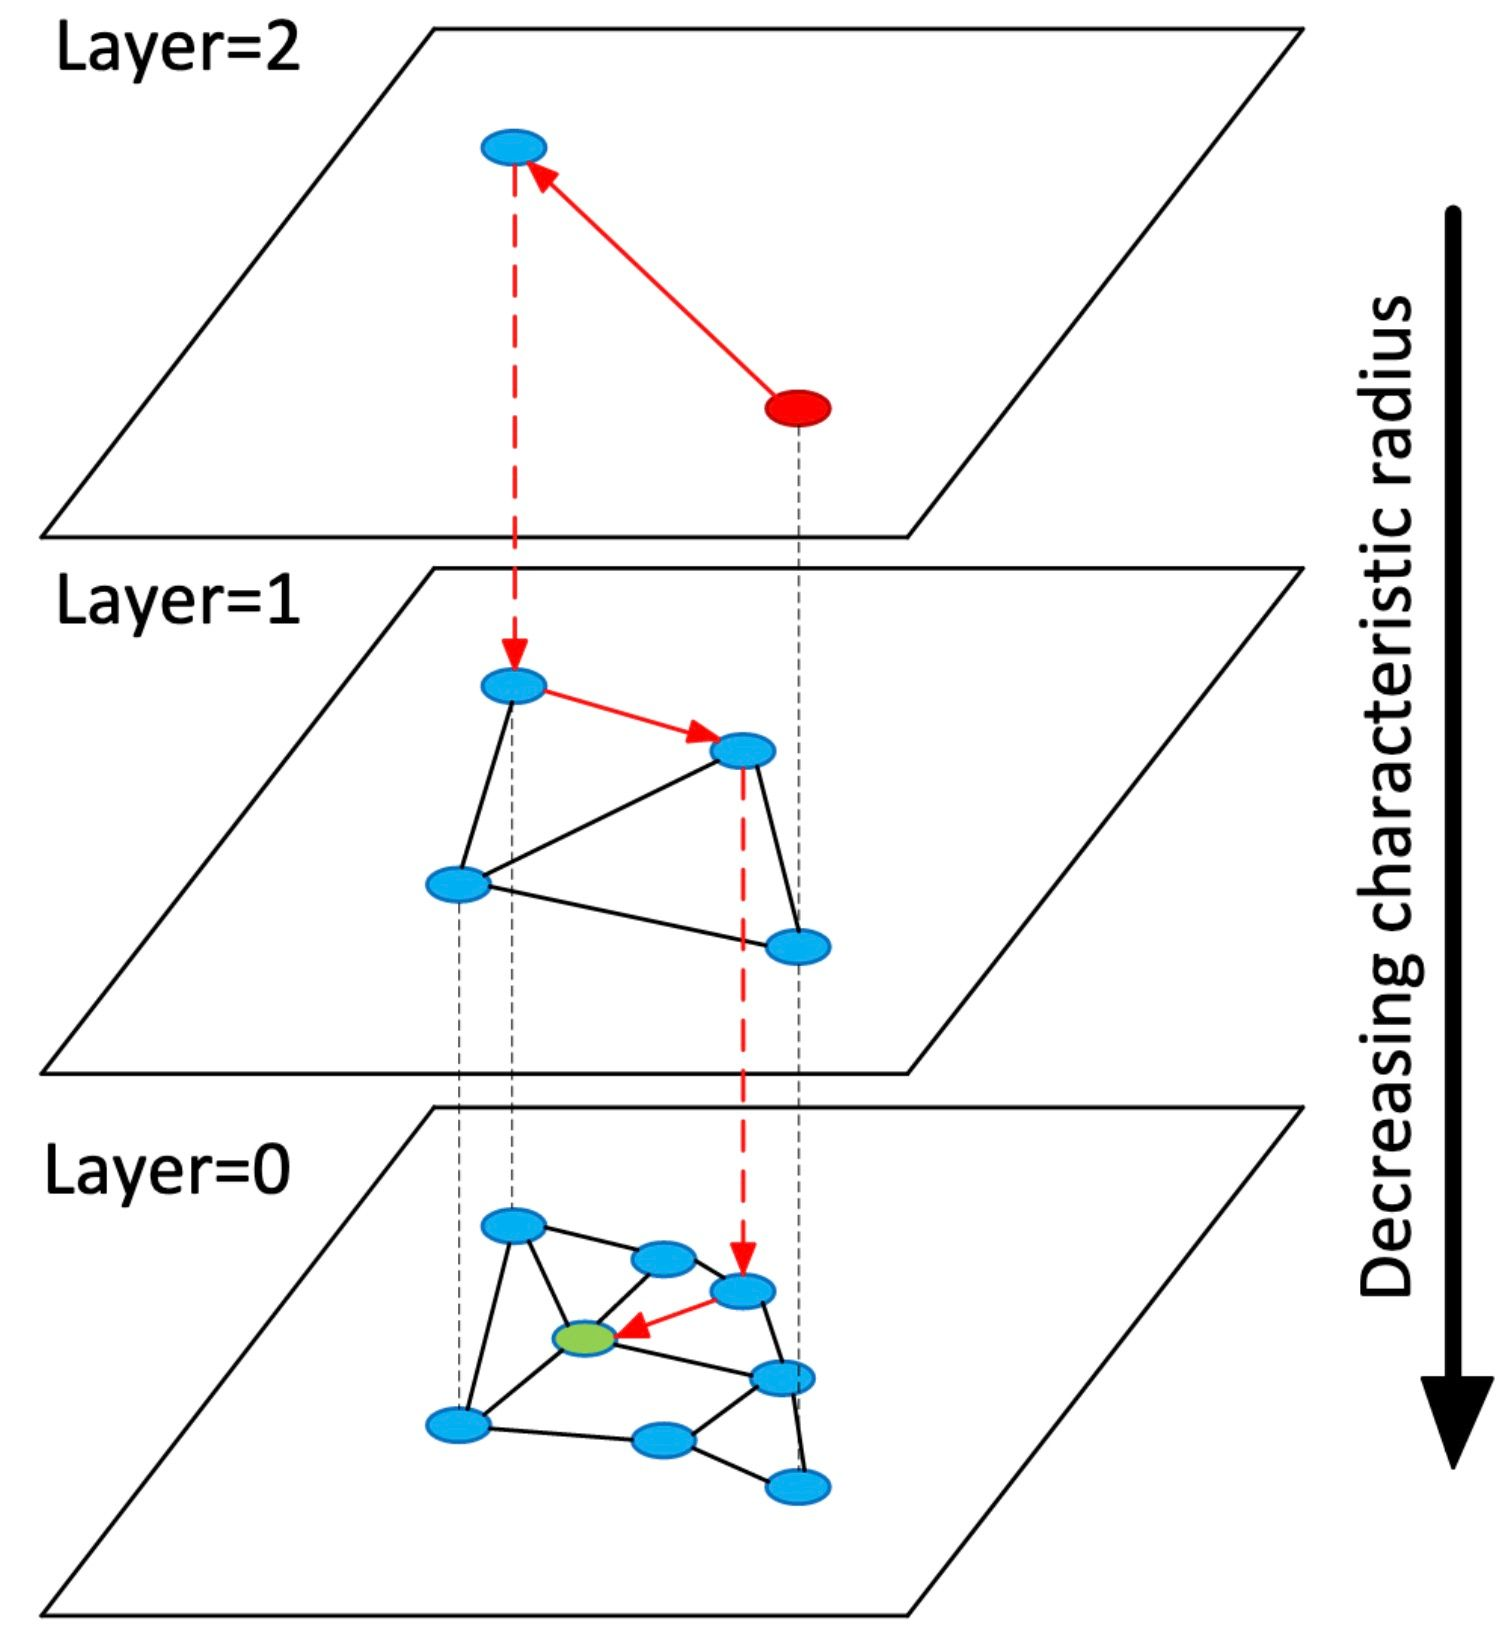
\includegraphics[width=0.3\textwidth]{images/hnsw_layers.jpg}
    \caption{
    Τα ανώτερα επίπεδα περιέχουν λιγότερους κόμβους, ενώ το επίπεδο 0 περιλαμβάνει όλα τα δεδομένα.}
\label{fig:hnsw_structure}
\end{figure}


Η ανάθεση των κόμβων στα επίπεδα πραγματοποιείται με τυχαίο τρόπο, σύμφωνα με μία γεωμετρική κατανομή. 
Με τον τρόπο αυτό, οι περισσότεροι κόμβοι εμφανίζονται μόνο στα χαμηλά επίπεδα, ενώ λίγοι κόμβοι φτάνουν στα ανώτερα επίπεδα, δημιουργώντας μία ιεραρχική δομή που διευκολύνει τη γρήγορη πλοήγηση στον γράφο.

Κάθε κόμβος συνδέεται με περιορισμένο αριθμό γειτόνων σε κάθε επίπεδο, σύμφωνα με ένα προκαθορισμένο όριο συνδεσιμότητας. 
Η δομή αυτή επιτρέπει την αποδοτική αναζήτηση, καθώς η πλοήγηση ξεκινά από τα ανώτερα επίπεδα και σταδιακά κατεβαίνει προς τα χαμηλότερα, προσεγγίζοντας ολοένα και πιο κοντινά σημεία στο ερώτημα.


\subsubsection{Διαδικασία Εισαγωγής Νέου Κόμβου}
Αρχικά για κάθε νέο κόμβο επιλέγεται τυχαία το επιπέδο στο οποίο θα ενταχθεί ο κόμβος. Η επιλογή αυτή γίνεται με τέτοιο τρόπο ώστε οι περισσότεροι κόμβοι να τοποθετούνται μόνο στα χαμηλά επίπεδα, ενώ λίγοι κόμβοι να εμφανίζονται και στα ανώτερα, δημιουργώντας μία ιεραρχία.

Στη συνέχεια, η διαδικασία ξεκινά από το ανώτερο επίπεδο του γράφου και πραγματοποιεί μία άπληστη αναζήτηση για τον εντοπισμό της κατάλληλης περιοχής σύνδεσης του νέου κόμβου. Η αναζήτηση αυτή επαναλαμβάνεται διαδοχικά σε κάθε επίπεδο, κατεβαίνοντας προς τα χαμηλότερα επίπεδα, μέχρι να φτάσει στο επίπεδο μηδέν.

Σε κάθε επίπεδο, ο νέος κόμβος συνδέεται με περιορισμένο αριθμό γειτονικών κόμβων, σύμφωνα με προκαθορισμένους κανόνες επιλογής γειτόνων. Οι περιορισμοί αυτοί εξασφαλίζουν ότι ο γράφος παραμένει αραιός και ότι η πλοήγηση κατά την αναζήτηση παραμένει αποδοτική

Συνοπτικά, η διαδικασία εισαγωγής περιλαμβάνει τα εξής βασικά βήματα:
\begin{itemize}
    \item Τυχαία επιλογή του ανώτερου επιπέδου εμφάνισης του κόμβου.
    \item Εκκίνηση αναζήτησης από το ανώτερο επίπεδο του γράφου.
    \item Σταδιακή κάθοδος στα χαμηλότερα επίπεδα με άπληστη αναζήτηση.
    \item Σύνδεση με περιορισμένο αριθμό γειτονικών κόμβων σε κάθε επίπεδο.
\end{itemize}

\subsubsection{Διαδικασία Αναζήτησης}
Η αναζήτηση πραγματοποιείται σε δύο διακριτές φάσεις: μία αρχική φάση γρήγορης προσέγγισης\selectlanguage{english}\texttt{(Greedy Search)}\selectlanguage{greek} στα ανώτερα επίπεδα κα μία τελική φάση λεπτομερούς αναζήτησης 

\paragraph{\selectlanguage{english}\texttt{Greedy Search:}\selectlanguage{greek}}
Στα ανώτερα επίπεδα του γράφου εφαρμόζεται αυτή η διαδικασία, με στόχο τον γρήγορο εντοπισμό μίας περιοχής του χώρου κοντά στο \selectlanguage{english}query.\selectlanguage{greek}
Η αναζήτηση ξεκινά από ένα αρχικό κόμβο εισόδου και σε κάθε βήμα εξετάζονται οι γειτονικοί κόμβοι επιλέγοντας εκείνον που βρίσκεται πιο κοντά στο ερώτημα σύμφωνα με το επιλεγμένο μέτρο απόστασης.

Η διαδικασία συνεχίζεται έως ότου δεν υπάρχει γειτονικός κόμβος που να βελτιώνει την απόσταση από το ερώτημα.

\paragraph{\selectlanguage{english}\texttt{Best-first Search:}\selectlanguage{greek}}
Αφού ολοκληρωθεί η αναζήτηση στα ανώτερα επίπεδα. η αναζήτηση συνεχίζεται στο \textbf{επίπεδο 0} του γράφου. Εδώ ο γράφος περιέχει όλα τα δεδομένα και χρησιμοποιείται η \selectlanguage{english}best-first search.\selectlanguage{greek}
Κατά τη διάρκεια της αναζήτησης διατηρείται ένα σύνολο υποψηφίων που ενημερώνονται συνεχώς με βάση την απόσταση τους από το \selectlanguage{english}query\selectlanguage{greek} και επιστρέφει ένα συγκεκριμένο αριθμό \textbf{\texttt{K}} κοντινότερων γειτόνων.



\subsubsection{Παράμετροι του Αλγορίθμου}

\begin{table}[H]
    \centering
    \caption{Βασικές παράμετροι του αλγορίθμου \selectlanguage{english}HNSW\selectlanguage{greek} και ο ρόλος τους \cite{malkov2018hnsw}}
    \label{tab:hnsw_params}
    \begin{tabular}{p{3cm} p{7cm} p{4cm}}
    \toprule
    \textbf{Παράμετρος} & \textbf{Περιγραφή} & \textbf{Επίδραση στη απόδοση} \\
    \midrule
    $M$ & Μέγιστος αριθμός γειτόνων που διατηρεί κάθε κόμβος σε κάθε επίπεδο του γράφου & Μεγαλύτερο $Μ$ αυξάνει την ακρίβεια, αλλά και τη χρήση μνήμης \\
    \midrule
    \selectlanguage{english}$efConstruction$\selectlanguage{greek} & Μέγεθος του συνόλου υποψήφιων κόμβων κατά τη διαδικασία εισαγωγής νέων στοιχείων & Υψηλότερη τιμή οδηγεί σε καλύτερη ποιότητα γράφου, αλλά αυξάνει  τον χρόνο κατασκευής \\
    \midrule
    \selectlanguage{english}$efSearch$\selectlanguage{greek} & Μέγεθος του συνόλου υποψήφιων κόμβων κατα τη διαδικασία αναζήτησης & Μεγαλύτερη τιμή αυξάνει την ακρίβεια αναζήτησης με κόστος μεγαλύτερου χρόνου \\
    \bottomrule
    \end{tabular}
\end{table}

\subsection{Συμβιβασμός Ακρίβειας και Κόστους (Accuracy--Cost Trade-off)}

Κάθε μέθοδος ANN έχει κάπου κρυμμένη μια ρύθμιση που ελέγχει πόσο «σκληρά» δουλεύει. Στον HNSW αυτή η ρύθμιση είναι η \selectlanguage{english}$ef_{\text{search}}$\selectlanguage{greek}. Μεγαλύτερη τιμή σημαίνει περισσότεροι υπολογισμοί απόστασης, αλλά και υψηλότερο \selectlanguage{english}Recall@k\selectlanguage{greek}. Μικρότερη τιμή — πιο γρήγορος αλγόριθμος, λιγότερο αξιόπιστος.

Η σχέση αυτή είναι μονοτονική: όσο αυξάνεται το \selectlanguage{english}effort\selectlanguage{greek}, τόσο μεγαλύτερη η πιθανότητα να βρεθούν οι σωστοί γείτονες. Αλλά η κλίση της καμπύλης δεν είναι σταθερή — σε κάποιο σημείο η βελτίωση σταματά να δικαιολογεί το επιπλέον κόστος.

Το πρόβλημα: μια σταθερή τιμή \selectlanguage{english}$ef_{\text{search}}$\selectlanguage{greek} για όλα τα ερωτήματα αγνοεί το γεγονός ότι δεν είναι όλα εξίσου δύσκολα. Ορισμένα ερωτήματα βρίσκουν τους γείτονές τους σε λίγα βήματα· άλλα απαιτούν εκτενή εξερεύνηση. Μια παράμετρος «one-size-fits-all» αναγκαστικά σπαταλά υπολογισμούς στα εύκολα ερωτήματα, ή θυσιάζει ακρίβεια στα δύσκολα.

\subsection{Δυσκολία ερωτήματος \selectlanguage{english}(Query Difficulty)\selectlanguage{greek}}
Η «δυσκολία» ενός ερωτήματος δεν είναι κάτι που μπορείς να ξέρεις πριν αρχίσεις να αναζητάς. Αλλά κατά τη διάρκεια της αναζήτησης, κάποια σήματα αρχίζουν να εμφανίζονται:
\begin{itemize}
    \item ο ρυθμός βελτίωσης των καλύτερων υποψηφίων — αν βελτιώνονται γρήγορα, το ερώτημα είναι πιθανώς εύκολο
    \item η σταθερότητα του συνόλου των \selectlanguage{english}$k$\selectlanguage{greek} καλύτερων γειτόνων — αν δεν αλλάζει για αρκετά βήματα, ίσως δεν αξίζει να συνεχίσεις
    \item η διαφορά απόστασης μεταξύ του καλύτερου και του $k$-οστου αποτελέσματος — μικρή διαφορά υποδηλώνει ότι βρίσκεσαι ήδη σε καλή περιοχή
\end{itemize}
Αυτά τα σήματα δεν είναι εγγυήσεις — αλλά αρκούν για να δικαιολογήσουν μια προσαρμοστική στρατηγική. Άλλωστε, ακόμα κι ένα ατελές κριτήριο τερματισμού μπορεί να εξοικονομεί σημαντικό χρόνο αν εφαρμόζεται στο σωστό σημείο.

\subsection{Προσαρμοστικές Στρατηγικές Αναζήτησης}
Ο συμβιβασμός ακρίβειας--κόστους έχει οδηγήσει σε δύο διαφορετικές φιλοσοφικές κατευθύνσεις:

\subsubsection{Προσαρμοστική Ρύθμιση του \selectlanguage{english}$ef_{\text{search}}$}
Αντί να χρησιμοποιείται σταθερό \selectlanguage{english}$ef_{\text{search}}$\selectlanguage{greek} για όλα τα ερωτήματα, η προσέγγιση αυτή επιλέγει διαφορετικό \selectlanguage{english}budget\selectlanguage{greek} ανά ερώτημα — εκτός αναζήτησης (\selectlanguage{english}offline\selectlanguage{greek}) ή κατά τη διάρκειά της. Απλά ερωτήματα παίρνουν μικρό \selectlanguage{english}budget\selectlanguage{greek}, δύσκολα παίρνουν μεγαλύτερο.

\subsubsection{Πρόωρος Τερματισμός \selectlanguage{english}(Early Termination)\selectlanguage{greek}}
Εδώ το \selectlanguage{english}budget\selectlanguage{greek} δεν ορίζεται εκ των προτέρων — η αναζήτηση απλώς σταματά όταν παρατηρεί σύγκλιση. Κριτήρια όπως η σταθεροποίηση των καλύτερων γειτόνων ή η στασιμότητα της καλύτερης απόστασης χρησιμεύουν ως σήμα τερματισμού. Η προσέγγιση είναι ελκυστική γιατί δεν απαιτεί \selectlanguage{english}calibration\selectlanguage{greek} — αλλά το κριτήριο πρέπει να είναι αρκετά αξιόπιστο για να μην θυσιάζει ακρίβεια.

\subsection{Ορισμός Υπολογιστικού Κόστους}

Σε όλα τα πειράματά μας, το κόστος αναζήτησης εκφράζεται ως αριθμός υπολογισμών απόστασης ανά ερώτημα — όχι ως χρόνος εκτέλεσης. Η επιλογή αυτή δεν είναι τυχαία: ο χρόνος εξαρτάται από το υλικό, την υλοποίηση και άλλους εξωγενείς παράγοντες, ενώ οι υπολογισμοί απόστασης είναι αντικειμενικοί και συγκρίσιμοι μεταξύ μεθόδων. Επίσης, για δεδομένη υλοποίηση, συσχετίζονται άμεσα με τον πραγματικό χρόνο εκτέλεσης.

Ο στόχος είναι η ελαχιστοποίηση αυτού του αριθμού, με δεδομένο ότι το \selectlanguage{english}recall\selectlanguage{greek} παραμένει αποδεκτό.
% =======================================
% ΥΛΟΠΟΙΗΣΗ ΑΛΓΟΡΙΘΜΟΥ HNSW: ΚΕΦΑΛΑΙΟ 3
% =======================================
\newpage
\section{Υλοποίηση του Αλγορίθμου \selectlanguage{english}HNSW}

Στο κεφάλαιο αυτό περιγράφεται η δική μας υλοποίηση του \selectlanguage{english}\textbf{HNSW}\selectlanguage{greek} — αυτή που χρησιμοποιείται ως \selectlanguage{english}Baseline\selectlanguage{greek} σε όλα τα πειράματα. Η υλοποίηση δεν στοχεύει να είναι η πιο γρήγορη δυνατή· στόχος ήταν να ακολουθεί πιστά τη θεωρητική περιγραφή του αλγορίθμου και να επιτρέπει εύκολη επέκταση για τις προσαρμοστικές παραλλαγές που εξετάζουμε στο επόμενο κεφάλαιο.

\subsection{Γενική Αρχιτεκτονική Υλοποίησης}
Η υλοποίηση είναι γραμμένη σε \selectlanguage{english}C++\selectlanguage{greek} και εκτίθεται στην \selectlanguage{english}Python\selectlanguage{greek} μέσω \selectlanguage{english}pybind11\selectlanguage{greek}. Στον σχεδιασμό της δώσαμε προτεραιότητα στη σαφήνεια έναντι της ακατέργαστης απόδοσης — αντίθετα με βιβλιοθήκες παραγωγικής χρήσης όπως το \selectlanguage{english}FAISS\selectlanguage{greek}, ο κώδικας δεν έχει \selectlanguage{english}SIMD\selectlanguage{greek} ή \selectlanguage{english}cache-tuned\selectlanguage{greek} εσωτερικά. Αυτή η επιλογή έχει κόστος σε \selectlanguage{english}QPS\selectlanguage{greek} — κόστος που φαίνεται στα πειράματα του Κεφαλαίου 5 — αλλά διευκολύνει σημαντικά την τροποποίηση της λογικής αναζήτησης χωρίς να χρειάζεται να αγγίξουμε χαμηλού επιπέδου βελτιστοποιήσεις.

Ο κώδικας οργανώνεται σε τρία ξεχωριστά κομμάτια: τις δομές δεδομένων του γράφου, τη διαδικασία εισαγωγής κόμβων και τη διαδικασία αναζήτησης.


\subsection{Δομές Δεδομένων}
Η υλοποίηση οργανώνεται γύρω από τις ακόλουθες δομές:
\begin{itemize}
    \item \textbf{Αποθήκευση διανυσμάτων:} πίνακας \selectlanguage{english}$N \times d$\selectlanguage{greek} (\selectlanguage{english}contiguous\selectlanguage{greek}) για αποδοτική πρόσβαση και υπολογισμό αποστάσεων.
    \item \textbf{Επίπεδα κόμβων:} για κάθε κόμβο αποθηκεύεται το μέγιστο επίπεδο στο οποίο εμφανίζεται.
    \item \textbf{Λίστες γειτόνων ανά επίπεδο:} για κάθε κόμβο και κάθε επίπεδο \selectlanguage{english}$l$\selectlanguage{greek} αποθηκεύετια λίστα από \selectlanguage{english}node ids\selectlanguage{greek} 
    \item \selectlanguage{english}\textbf{Visited:}\selectlanguage{greek} δομή για αποφυγή επανεπίσκεψης κόμβων κατά την αναζήτηση.
    \item \textbf{Ουρές προτεραιότητας:} μία για υποψηφίου προς επέκταση και μία για το τρέχον σύνολο αποτελεσμάτων (μέχρι \selectlanguage{english}$ef_{\text{search}}$\selectlanguage{greek})
\end{itemize}
Ο διαχωρισμός \selectlanguage{english}candidate queue\selectlanguage{greek} και \selectlanguage{english}top set\selectlanguage{greek} είναι κρίσιμος, καθώς επιτρέπει τον έλεγχο του search effort μέσω του \selectlanguage{english}$ef_{\text{search}}$\selectlanguage{greek} και αποτελεί τη βάση για τις προσαρμοστικές βελτιώσεις του επόμενου κεφαλαίου.

\subsection{Εισαγωγή Νέου Κόμβου}
Η εισαγωγή ενός νέου κόμβου (διανύσματος) στο \selectlanguage{english}\texttt{HNSW}\selectlanguage{greek} πραγματοποιείται σταδιακά από τα ανώτερα επίπεδα προς το επίπεδο βάσης (\selectlanguage{english}level 0\selectlanguage{greek}), ώστε ο κόμβος να ενσωματωθεί στη ιεραρχική δομή του γράφου και να δημιουργηθούν οι κατάλληλες ακμές σύνδεσης.

\subsubsection{Ανάθεση επιπέδου (\selectlanguage{english}Layer Assignment\selectlanguage{greek})}
Κάθε νέος κόμβος $q$ ανατίθεται σε ένα  επίπεδο $L$\selectlanguage{english} (layer),\selectlanguage{greek} αυτη η ανάθεση επιπέδου γίνεται τυχαία, ακολουθώντας εκθετική/γεωμετρική κατανομή ώστε τα ανώτερα επίπεδα να είναι πιο αραιά και λιγότερα σχέση με τα υπόλοιπα επίπεδα. Συγκεκριμένα:
\begin{equation}
    P(L \ge l) = e^{-l/\lambda}
\end{equation}
όπου $\lambda$ παράμετρος κλίμακας (όπου στην πράξη συνδέεται με το $Μ$, δηλαδή το μέγιστο πλήθος γειτόνων ανά επίπεδο). Συγκεκριμένα.
\begin{equation}
    \lambda = \frac{1}{\ln{M}}
\end{equation}
\subsubsection{\selectlanguage{english}Greedy\selectlanguage{greek} πλοήγηση στα ανώτερα επίπεδα}
ξεκινώντας από έναν κόμβο εισόδου $c$ στο ανώτερο διαθέσιμο επίπεδο, εκτελείται \selectlanguage{english}greedy\selectlanguage{greek}.Στο επίπεδο $l$, η ενημέρωση του τρέχον κόμβου μπορεί να εκφραστεί ως:
\begin{equation}
    c \leftarrow \arg\min_{v \in \mathcal{N}_l(c)} d(q,v),
\end{equation}
όπου $\mathcal{N}_l(c)$ είναι οι γείτονες του $c$ στο επίπεδο $l$ και $d(\cdot,\cdot)$ η μετρική απόσταση που χρησιμοποιούμε

\subsubsection{Αναζήτηση υποψηφίων στο επίπεδο βάσης (\selectlanguage{english}level 0\selectlanguage{greek})}
Στο επίπεδο βάσης δεν αρκεί η \selectlanguage{english}greedy search\selectlanguage{greek} διαδικασία, καθώς απαιτείται καλύτερη τοπική διερεύνηση για να δημιουργηθεί ποιοτικός γράφος. Για τον λόγο αυτό εφαρμόζεται αναζήτηση τύπου \selectlanguage{english}best-first search\selectlanguage{greek}, με παράμετρο \selectlanguage{english}$ef_{\text{construction}}$\selectlanguage{greek}, η οποία ελέγχει πόσους υποψήφιους κόμβους διατηρούμε κατά την κατασκευή


\subsubsection{Επιλογή γειτόνων και δημιουργία ακμών}
Από το σύνολο των υποψηφίων κόμβων στο επίπεδο $l$ επιλέγχονται έως $Μ$ γείτονες για να συνδεθεί ο νέος κόμβος $q$. Η επιλογή δεν γίνεται μόνο με βάση την ελάχιστη απόσταση από το $q$, αλλά εφαρμόζεται \selectlanguage{english}heuristic\selectlanguage{greek} που ενισχύει την ποικιλομορφία των ακμών και αποφεύγει πλεονάζουσες συνδέσεις.

Ένα τυπικό κριτήριο αποδοχής ενός υποψηφίου $u$ στο σύνολο επιλεγμένων γειτόνων $S$ είναι:
\begin{equation}
    \forall w \in S:\quad d(u,q) < d(u,w)
\end{equation}
δηλαδή ο $u$ γίνεται δεκτός μόνο αν δεν ``καλύπτεται'' από κάποιον ήδη επιλεγμένο γείτονα $w$.
Τέλος, οι ακμές εισάγονται αμφίδρομα (\selectlanguage{english}bidirectional links\selectlanguage{greek}) μεταξύ $q$ και των επιλεγμένων
γειτόνων, ενώ αν σε κάποιον κόμβο υπερβεί το πλήθος γειτόνων το επιτρεπτό όριο, εφαρμόζεται τοπικό
\selectlanguage{english}pruning\selectlanguage{greek}.
\medskip
Η παραπάνω διαδικασία επαναλαμβάνεται για όλα τα επίπεδα  $l \le L$ στα οποία ανήκει ο κόμβος $q$, επιτυγχάνοντας σταδιακή ενσωμάτωση του νέου κόμβου στον ιεραρχικό γράφο.

\subsection{Αναζήτηση \selectlanguage{english}(Querying)}
Η διαδικασία αναζήτησης στο \selectlanguage{english}HNSW\selectlanguage{greek} έχει ως στόχο την εύρεση των $k$ πλησιέστερων γειτόνων ενός ερωτήματος $q$, εκμεταλλευόμενη τη ιεραρχική δομή του γράφου ώστε να επιτυγχάνεται αποδοτικός προσεγγιστικός εντοπισμός κοντινών κόμβων.

Η αναζήτηση πραγματοποιείται σε δύο διακριτά στάδια:
\begin{itemize}
    \item πλοήγηση στα ανώτερα επίπεδα του γράφου και 
    \item λεπτομερής αναζήτηση στο επίπεδο βάσης
\end{itemize}

\subsubsection{Πλοήγηση στα ανώτερα επίπεδα}
Η διαδικασία ξεκινά από έναν κόμβο εισόδου $c$ στο ανώτερο επίπεδο του γράφου. Σε κάθε επίπεδο $l$, εφαρμόζεται \selectlanguage{english}greedy search,\selectlanguage{greek} κατά την οποία ο τρέχων κόμβος ενημερώνεται επιλέγοντας τον γείτονα που ελαχιστοποιεί την απόσταση από το ερώτημα $q$:
\begin{equation}
    c \leftarrow \arg\min_{v \in \mathcal{N}_l(c)} d(q,v)
\end{equation}
όπου $\mathcal{N}_l(c)$ είναι το σύνολο των γειτόνων του $c$ στο επίπεδο $l$. Η διαδικασία αυτή επαναλαμβάνεται μέχρι να μην υπάρχει γείτονας που να βελτιώνει την απόσταση από το $q$, οπότε η αναζήτηση συνεχίζεται στο αμέσως κατώτερο επίπεδο.

Ο σκοπός αυτού του σταδίου είναι ο γρήγορος εντοπισμός μιας καλής αρχικής περιοχής του γράφου κοντά στο ερώτημα, χωρίς εκτενήη διερεύνηση.

\subsubsection{Αναζήτηση στο επίπεδο βάσης (\selectlanguage{english}level 0\selectlanguage{greek})}
Στο επίπεδο βάσης εφαρμόζεται αναζήτηση τύπου \selectlanguage{english}best-first\selectlanguage{greek}
Η υλοποίηση διατηρεί δύο δομές:
\begin{enumerate}
    \item μία ουρά υποψηφίων προς επέκταση (\selectlanguage{english}candidate queue\selectlanguage{greek})
    \item ένα σύνολο των καλύτερων κόμβων που έχουν βρεθεί μέχρι στιγμής (\selectlanguage{english}top set\selectlanguage{greek}) μεγέθους έως \selectlanguage{english}$ef_{\text{search}}$\selectlanguage{greek}.
\end{enumerate}
Σε κάθε βήμα επιλέγεται προς επέκταση ο υποψήφιος με τη μικρότερη απόσταση από το ερώτημα \selectlanguage{english}$q$\selectlanguage{greek}.
Οι γείτονες του εξετάζονται και εισάγονται στο \selectlanguage{english}top set\selectlanguage{greek} εφόσον βελτιώνουν την τρέχουσα λίστα των καλύτερων αποτελεσμάτων.

Η διαδικασία τερματίζεται όταν ο καλύτερος διαθέσιμος υποψήφιος προς επέκταση είναι χειρότερος από τον χειρότερο κόμβο στο \selectlanguage{english}top set\selectlanguage{greek}, δηλαδή όταν:
\[
d\bigl(q,v_{\text{best cand}}\bigr) > d\bigl(q,v_{\text{worst in top}}\bigr)
\]
Ο κανόνας αυτός εξασφαλίζει ότι περαιτέρω επεκτάσεις είναι απίθανο να βελτιώσουν το τρέχον σύνολο των καλύτερων υποψηφίων

\subsubsection{Εξαγωγή αποτελεσμάτων}
Με την ολοκλήρωση της αναζήτησης στο επίπεδο βάσης, το σύνολο των υποψηφίων κόμβων ταξινομείται με βάση την απόστασή τους από το ερώτημα $q$ και επιστρέφονται οι $k$ πλησιέστεροι κόμβοι ως αποτέλεσμα της αναζήτησης.

Η παράμετρος $ef_{\text{search}}$ επηρεάζει άμεσα τον συμβιβασμό μεταξύ ακρίβειας και χρόνου αναζήτησς: μεγαλύτερες τιμές οδηγούν σε υψηλότερο \selectlanguage{english}recall\selectlanguage{greek}, με αυξημένο υπολογιστικό κόστος.

\subsection{Διαχείριση Μνήμης και Πολυπλοκότητα}
\subsection{Καταγραφή Μετρικών Κόστους (\selectlanguage{english}Instrumentation\selectlanguage{greek})}
Για την αξιολόγηση τόσο της βασικής υλοποίησης όσο και των προτεινόμενων βελτιώσεων, καταγράφονται μετρικές κόστους κατά την αναζήτηση:
\begin{itemize}
    \item \textbf{Αριθμός υπολογισμών απόστασης} ανά ερώτημα (\selectlanguage{english}\#distance computations\selectlanguage{greek}).
    \item \textbf{Αριθμός επεκτάσεων κόμβων} (\selectlanguage{english}node expansions\selectlanguage{greek}) στο επίπεδο 0.
    \item \textbf{Χρόνος αναζήτησης} (σε ms), ως δευτερεύουσα μετρική που εξαρτάται από την υλοποίηση και το υλικό.
\end{itemize}
Η μετρική \selectlanguage{english}\#distance computations\selectlanguage{greek} θεωρείται η βασική, καθώς είναι \selectlanguage{english}hardware-agnostic\selectlanguage{greek} και συσχετίζεται άμεσα με τον χρόνο εκτέλεσης.

\subsubsection{Δομές δεδομένων και χρήση μνήμης}
Κάθε κόμβος του γράφου αποθηκεύει:
\begin{itemize}
    \item το διάνυσμα χαρακτηριστικών του
    \item τη μέγιστη στάθμη \selectlanguage{english}(level)\selectlanguage{greek} στην οποία ανήκει
    \item λίστες γειτόνων για κάθε επίπεδο στο οποίο εμφανίζεται
\end{itemize}

Στο επίπεδο $l$, ο μέγιστος αριθμός γειτόνων ανά κόμβο περιορίζεται από την παράμετρο $M_l$ (στην πράξη $M_l$ για $l>0$ και $M_0 \ge M$ για το επίπεδο βάσης). Επομένως, η μνήμη που απαιτείται για την αποθήκευση των ακμών του γράφου είνια της τάξης:
\begin{equation}
    \mathcal{O}(N\cdot M)
\end{equation}
όπου $Ν$ το πλήθος των κόμβων του index.

Η ιεραρχική κατανομή των κόμβων στα επίπεδα εξασφαλίζει ότι ο συνολικός αριθμός επιπέδων αυξάνεται λογαριθμικά ως προς το $Ν$, με αποτέλεσμα το επιπλέον κόστος μνήμης λόγω των ανώτερων επιπέδων να παραμένει περιορισμένο.

\subsubsection{Πολυπλοκότητα εισαγωγής κόμβου}
Η εισαγωγή ενός νέου κόμβου περιλαμβάνει:
\begin{enumerate}
    \item \selectlanguage{english}greedy\selectlanguage{greek} πλοήγηση στα ανώτερα επίπεδα
    \item αναζήτηση τύπου \selectlanguage{english}best-first\selectlanguage{greek} στο επίπεδο βάσης με εύρος \selectlanguage{english} $ef_{\text{construction}}$\selectlanguage{greek}
    \item επιλογή και σύνδεση έως $Μ$ γειτόνων ανά επίπεδο
\end{enumerate}

Υπό την παραδοχή ότι το πλήθος των επιπέδων αυξάνεται λογαριθμικά, το αναμενόμενο κόστος εισαγωγής ενός κόμβου κυριαρχείται από την αναζήτηση στο επίπεδο βάσης και εξαρτάται γραμμικά από το \selectlanguage{english}$ef_{\text{construction}}$\selectlanguage{greek}. Στην πράξη, μεγαλύτερες τιμές του
\selectlanguage{english}$ef_{\text{construction}}$\selectlanguage{greek} οδηγούν σε καλύτερη ποιότητα γράφου, με αυξημένο όμως χρόνο κατασκευής

\subsubsection{Πολυπλοκότητα αναζήτησης}
Η διαδικασία αναζήτησης αποτελείται από:
\begin{itemize}
    \item \selectlanguage{english}greedy\selectlanguage{greek} πλοήγηση στα ανώτερα επίπεδα
    \item \selectlanguage{english}best-first search\selectlanguage{greek} στο επίπεδο βάσης με παράμετρο \selectlanguage{english}$ef_{\text{search}}$\selectlanguage{greek}
\end{itemize}
Το κόστος της αναζήτησς καθορίζεται κυρίως από τον αριθμό υπολογισμών απόστασης που εκτελούνται στο επίπεδο βάσης, ο οποίος αυξάνεται με το \selectlanguage{english}$ef_{\text{search}}$\selectlanguage{greek}. Έτσι, ο \selectlanguage{english}HNSW\selectlanguage{greek} προσφέρει έναν άμεσο μηχανισμό ελέγχου του συμβιβασμού μεταξύ χρόνου και ακρίβειας αναζήτησης, ρυθμίζοντας την τιμή της \selectlanguage{english}$ef_{\text{search}}$\selectlanguage{greek}

\subsubsection{Σχόλια για αποδοτικότητα και επεκτασιμότητα}
Η σχεδίαση του \selectlanguage{english}HNSW\selectlanguage{greek} επιτρέπει:
\begin{itemize}
    \item αποδοτική αναζήτηση με υπο-γραμμική συμπεριφορά ως προς το $N$,
    \item δυναμική εισαγωγή νέων κόμβων χωρίς ανακατασκευή του \selectlanguage{english}index\selectlanguage{greek}
    \item έλεγχο του κόστους μέσω των παραμέτρων $Μ$, \selectlanguage{english}$ef_{\text{construction}}$\selectlanguage{greek} και \selectlanguage{english}$ef_{\text{search}}$\selectlanguage{greek}
\end{itemize}
Ωστόσο, η απόδοση του αλγορίθμου εξαρτάται σε μεγάλο βαθμό από τις επιλεγμένες τιμές των παραμέτρων και τις ευρετικές επιλογής γειτόνων, γεγονός που δημιουργεί περιθώρια για περαιτέρω βελτιστοποίηση. 


\subsection{Testing της Υλοποίησης}


%Αdaptive efSearch + early stopping , neighbor selection in build 

%hnswlib , faiss hsnw, lucene hnsw , 

% I will see what i'm going to use and if i use more but for now i will keep this structure
% =======================================
% ΠΡΟΤΕΙΝΟΜΕΝΕΣ ΒΕΛΤΙΩΣΕΙΣ: ΚΕΦΑΛΑΙΟ 4 
% =======================================
\newpage

\section{Προτεινόμενη Βελτίωση}

\subsection{Κίνητρο}
Ξεκινώντας από τη βασική υλοποίηση του \selectlanguage{english}HNSW\selectlanguage{greek}, το πρώτο πράγμα που παρατηρεί κανείς είναι ότι η παράμετρος \selectlanguage{english}$ef_{\text{search}}$\selectlanguage{greek} είναι σταθερή — ίδια για κάθε ερώτημα που υποβάλλεται. Στην πράξη αυτό σημαίνει ότι ο αλγόριθμος αντιμετωπίζει ένα εύκολο ερώτημα (για το οποίο οι γείτονες βρίσκονται σχεδόν αμέσως) ακριβώς με τον ίδιο τρόπο που αντιμετωπίζει ένα δύσκολο. Δύο πιθανά προβλήματα προκύπτουν:
\begin{itemize}
    \item \textbf{Υπερβολική εξερεύνηση \selectlanguage{english}(over-searching)\selectlanguage{greek}:} για ερωτήματα που συγκλίνουν γρήγορα, η αναζήτηση συνεχίζεται άσκοπα — πληρώνεις υπολογισμούς που δεν αλλάζουν το αποτέλεσμα.
    \item \textbf{Ανεπαρκής εξερεύνηση \selectlanguage{english}(under-searching)\selectlanguage{greek}:} για δύσκολα ερωτήματα, μια χαμηλή σταθερή τιμή \selectlanguage{english}$ef_{\text{search}}$\selectlanguage{greek} κόβει την αναζήτηση πριν βρεθούν οι σωστοί γείτονες — και το \selectlanguage{english}recall\selectlanguage{greek} πέφτει.
\end{itemize}
Διαφορετικά ερωτήματα απαιτούν διαφορετικό βαθμό εξερεύνησης. Μια σταθερή παραμετροποίηση αδυνατεί να ικανοποιήσει και τις δύο περιπτώσεις ταυτόχρονα.

\subsection{Διατύπωση του Στόχου}
Ο στόχος είναι απλός στη διατύπωση: να ελαχιστοποιηθεί το υπολογιστικό κόστος ανά ερώτημα, με την προϋπόθεση ότι η ακρίβεια δεν πέφτει κάτω από ένα αποδεκτό κατώφλι.

\[
\min \; \text{Cost}(q)
\quad \text{υπό τον περιορισμό}\quad
\text{Recall@k}(q) \ge \tau
\]
όπου το κόστος μετριέται σε αριθμό υπολογισμών απόστασης και $\tau$ είναι ο επιθυμητός στόχος ακρίβειας.

Η διατύπωση αυτή είναι σημαντική γιατί αλλάζει το πλαίσιο: δεν ρωτάμε «πόσο υψηλό recall μπορούμε να πετύχουμε», αλλά «με πόσο κόστος μπορούμε να φτάσουμε ένα επαρκές recall». Αυτή η ερώτηση είναι πιο κοντά σε αυτό που απαιτούν τα πραγματικά συστήματα.

\subsection{Βασική Ιδέα}
Αντί να δεσμευόμαστε σε σταθερό \selectlanguage{english}$ef_{\text{search}}$\selectlanguage{greek} πριν αρχίσει η αναζήτηση, η κεντρική ιδέα είναι να παρακολουθούμε την πορεία της αναζήτησης και να αποφασίζουμε κατά τη διάρκειά της πότε έχουμε κάνει αρκετά. Με άλλα λόγια: αφήνουμε τα δεδομένα να πουν πόσο δύσκολο είναι το ερώτημα.

Τα σήματα που μπορούν να χρησιμοποιηθούν για αυτή την απόφαση:

\begin{itemize}
    \item ο ρυθμός βελτίωσης των καλύτερων αποστάσεων — αν σταματάει να βελτιώνεται, ίσως είμαστε ήδη κοντά στο βέλτιστο
    \item η σταθεροποίηση του συνόλου των \selectlanguage{english}$k$\selectlanguage{greek} καλύτερων γειτόνων — αν οι ίδιοι κόμβοι παραμένουν στην κορυφή για αρκετά βήματα, επιπλέον εξερεύνηση μάλλον δεν αλλάζει τίποτα
    \item η διαφορά μεταξύ της καλύτερης και της \selectlanguage{english}$k$\selectlanguage{greek}-οστής απόστασης — μικρή διαφορά σημαίνει «πυκνή» γειτονιά, άρα εύκολο ερώτημα
\end{itemize}

Αν αυτά τα σήματα δείχνουν σύγκλιση, η αναζήτηση μπορεί να τερματιστεί νωρίς. Ακόμα κι αν η απόφαση είναι ευριστική και όχι εγγυημένη, ακόμα κι ένα ατελές κριτήριο εξοικονομεί πόρους στα «εύκολα» ερωτήματα — που είναι πολλά στην πράξη.

\subsection{Σχέση με Υφιστάμενες Προσεγγίσεις}

Οι μέθοδοι που εξετάζουμε στην εργασία αυτή υλοποιούν αυτές τις ιδέες με αρκετά διαφορετικούς τρόπους.

Η \selectlanguage{english}DARTH\selectlanguage{greek} χρησιμοποιεί ένα μοντέλο \selectlanguage{english}LightGBM\selectlanguage{greek} που εκπαιδεύεται \selectlanguage{english}offline\selectlanguage{greek} για να προβλέπει πότε η αναζήτηση μπορεί να σταματήσει με ασφάλεια — δηλαδή χωρίς να χαθεί \selectlanguage{english}recall\selectlanguage{greek}. Η \selectlanguage{english}Ada-ef\selectlanguage{greek} παίρνει διαφορετική κατεύθυνση: ρυθμίζει το \selectlanguage{english}efSearch\selectlanguage{greek} ανά ερώτημα βασιζόμενη σε βαθμονόμηση \selectlanguage{english}offline\selectlanguage{greek} και \selectlanguage{english}cosine similarity\selectlanguage{greek}. Η \selectlanguage{english}PiP\selectlanguage{greek} επιλέγει εντελώς διαφορετική στρατηγική: αντί να σταματάει νωρίς, κλαδεύει υποψηφίους κατά την αναζήτηση χρησιμοποιώντας γεωμετρικό κριτήριο.

Κάθε μία από αυτές τις τρεις προσεγγίσεις αντιπροσωπεύει μια ξεχωριστή φιλοσοφία για το πώς να μειωθεί το κόστος αναζήτησης. Η σύγκρισή τους σε κοινή βάση — αυτό είναι που επιδιώκουμε στο κεφάλαιο των πειραμάτων.

\subsection{Αναμενόμενα Οφέλη και Περιορισμοί}
Θεωρητικά, η δυναμική ρύθμιση του \selectlanguage{english}search effort\selectlanguage{greek} μπορεί να μειώσει σημαντικά τον μέσο αριθμό υπολογισμών ανά ερώτημα — ιδιαίτερα όταν ένα μεγάλο ποσοστό ερωτημάτων είναι «εύκολα» και συγκλίνουν γρήγορα. Σε datasets με ετερογενή κατανομή δυσκολίας, το όφελος μπορεί να είναι εντυπωσιακό.

Στην πράξη όμως τα πράγματα εξαρτώνται από αρκετούς παράγοντες. Το κριτήριο τερματισμού πρέπει να είναι αρκετά αξιόπιστο ώστε να μην χάνει recall στα δύσκολα ερωτήματα — αν ενεργοποιείται πρόωρα, βλέπεις πτώση στην ακρίβεια. Επίσης, datasets με ομοιόμορφη κατανομή δεν αφήνουν πολλά περιθώρια: αν τα περισσότερα ερωτήματα είναι εξίσου δύσκολα, δεν υπάρχει τι να εξοικονομήσεις. Αυτό ακριβώς επιβεβαιώθηκε στα πειράματά μας με το \selectlanguage{english}GloVe-100\selectlanguage{greek}.
% =======================================
% ΠΕΙΡΑΜΑΤΑ ΚΑΙ ΑΞΙΟΛΟΓΗΣΗ: ΚΕΦΑΛΑΙΟ 5
% =======================================
\newpage
\section{\selectlanguage{greek}Πειράματα και Αξιολόγηση}

Στο κεφάλαιο αυτό παρουσιάζουμε τα αποτελέσματα της πειραματικής σύγκρισης των πέντε μεθόδων: \selectlanguage{english}Baseline-HNSW, DARTH, PiP, Ada-ef \selectlanguage{greek}και \selectlanguage{english}faiss-hnsw\selectlanguage{greek}. Αρχικά περιγράφονται τα σύνολα δεδομένων και οι μετρικές που χρησιμοποιήθηκαν, και στη συνέχεια παρουσιάζουμε τα αριθμητικά αποτελέσματα και τις παρατηρήσεις που προέκυψαν κατά τη διεξαγωγή των πειραμάτων.

\subsection{Σύνολα Δεδομένων}

Για την αξιολόγηση επιλέξαμε πέντε σύνολα δεδομένων που διαφέρουν αρκετά μεταξύ τους — τόσο σε μέγεθος και διάσταση, όσο και στη δομή των δεδομένων τους. Η επιλογή αυτή έγινε σκόπιμα, ώστε να ελεγχθεί αν οι μέθοδοι συμπεριφέρονται ομοιόμορφα ή αν εξαρτώνται από τα χαρακτηριστικά του εκάστοτε dataset. Ο Πίνακας~\ref{tab:datasets} δίνει μια σύνοψη.

\begin{table}[H]
\centering
\caption{Χαρακτηριστικά συνόλων δεδομένων}
\label{tab:datasets}
\begin{tabular}{lrrrr}
\toprule
\textbf{Dataset} & \textbf{Βάση (N)} & \textbf{Διάσταση (d)} & \textbf{Ερωτήματα} & \textbf{Μετρική} \\
\midrule
SIFT Small       & 10.000      & 128  & 100    & L2 \\
Fashion-MNIST    & 55.000      & 784  & 10.000 & L2 \\
MS MARCO Text    & 40.000      & 384  & 5.000  & L2 \\
GloVe-100        & 1.183.514   & 100  & 10.000 & L2 \\
SIFT-1M          & 1.000.000   & 128  & 10.000 & L2 \\
\bottomrule
\end{tabular}
\end{table}

\begin{itemize}
    \item \textbf{\selectlanguage{english}SIFT Small\selectlanguage{greek}:} Κλασικό μικρό σύνολο με περιγραφητές \selectlanguage{english}SIFT\selectlanguage{greek} από εικόνες. Το χρησιμοποιήσαμε κυρίως για γρήγορο έλεγχο ορθότητας — με μόλις 10.000 διανύσματα, τα αποτελέσματα βγαίνουν γρήγορα και μπορεί κανείς να εντοπίσει εύκολα λάθη.

    \item \textbf{\selectlanguage{english}Fashion-MNIST\selectlanguage{greek}:} Εικόνες ρούχων 784 διαστάσεων (εικόνες $28 \times 28$ \selectlanguage{english}pixels\selectlanguage{greek} απλωμένες σε διάνυσμα). Η υψηλή διάσταση σε σχέση με τον σχετικά μικρό αριθμό δεδομένων το κάνει ενδιαφέρον για να δούμε πώς επηρεάζεται η αναζήτηση.

    \item \textbf{\selectlanguage{english}MS MARCO Text\selectlanguage{greek}:} Διανύσματα κειμένου 384 διαστάσεων, παραγόμενα από ένα μοντέλο \selectlanguage{english}embedding\selectlanguage{greek} πάνω στο \selectlanguage{english}MS MARCO\selectlanguage{greek}. Το επιλέξαμε γιατί αντιπροσωπεύει πραγματικά σενάρια ανάκτησης πληροφορίας — το είδος δεδομένων που συναντάμε σε συστήματα \selectlanguage{english}RAG\selectlanguage{greek} και ανάλογες εφαρμογές.

    \item \textbf{\selectlanguage{english}GloVe-100\selectlanguage{greek}:} Διανύσματα λέξεων 100 διαστάσεων από το \selectlanguage{english}GloVe\selectlanguage{greek}, με 1.183.514 διανύσματα βάσης. Το επιλέξαμε επειδή η κατανομή του είναι αρκετά διαφορετική από τα \selectlanguage{english}SIFT\selectlanguage{greek}-based datasets — τα διανύσματα λέξεων τείνουν να είναι πιο ομοιόμορφα κατανεμημένα στον χώρο, κάτι που δυσκολεύει τη γραφο-αναζήτηση. Χρησιμοποιούμε ευκλείδεια απόσταση στα αρχικά (μη κανονικοποιημένα) διανύσματα.

    \item \textbf{\selectlanguage{english}SIFT-1M\selectlanguage{greek}:} Το πλήρες \selectlanguage{english}SIFT\selectlanguage{greek} dataset με 1.000.000 διανύσματα 128 διαστάσεων. Επιλέχθηκε για να εξεταστεί η κλιμακωσιμότητα των μεθόδων σε πραγματική κλίμακα παραγωγής, δεδομένου ότι τα datasets εκατομμυρίων διανυσμάτων είναι τυπικά σε σύγχρονες διανυσματικές βάσεις δεδομένων.
\end{itemize}

\subsection{Μετρικές Αξιολόγησης}

Οι δύο κεντρικές μετρικές που χρησιμοποιήθηκαν είναι το \selectlanguage{english}Recall@k\selectlanguage{greek} και το \selectlanguage{english}QPS\selectlanguage{greek}. Η επιλογή τους δεν είναι τυχαία — μαζί αποτυπώνουν ακριβώς τον βασικό συμβιβασμό που μας ενδιαφέρει: ακρίβεια έναντι ταχύτητας.

\subsubsection{\selectlanguage{english}Recall@k}
Το \selectlanguage{english}Recall@k\selectlanguage{greek} μετράει τι ποσοστό από τους πραγματικούς $k$ κοντινότερους γείτονες επέστρεψε ο αλγόριθμος:
\[
\text{Recall@}k = \frac{1}{n_q} \sum_{i=1}^{n_q} \frac{|\hat{N}_k(q_i) \cap N_k(q_i)|}{k}
\]
όπου $N_k(q_i)$ είναι οι πραγματικοί $k$ γείτονες του ερωτήματος $q_i$ (υπολογισμένοι εξαντλητικά) και $\hat{N}_k(q_i)$ αυτοί που επέστρεψε ο αλγόριθμος. Τιμή 1.0 σημαίνει τέλεια ακρίβεια.

\subsubsection{\selectlanguage{english}QPS (Queries Per Second)}
Το \selectlanguage{english}QPS\selectlanguage{greek} εκφράζει πόσα ερωτήματα επεξεργάζεται ο αλγόριθμος ανά δευτερόλεπτο — απλά, πόσο γρήγορος είναι. Όλες οι μετρήσεις έγιναν με ένα νήμα (\selectlanguage{english}single-threaded\selectlanguage{greek}), ώστε η σύγκριση να μην επηρεάζεται από διαφορές στην παραλληλοποίηση μεταξύ υλοποιήσεων.

\subsection{Πειραματική Διαδικασία}

\subsubsection{Περιβάλλον Εκτέλεσης}
Τα πειράματα τρέξαν σε μηχάνημα με \selectlanguage{english}Apple M1\selectlanguage{greek}, σε \selectlanguage{english}single-threaded\selectlanguage{greek} λειτουργία. Οι υλοποιήσεις \selectlanguage{english}Baseline-HNSW, DARTH\selectlanguage{greek} και \selectlanguage{english}PiP\selectlanguage{greek} είναι γραμμένες σε \selectlanguage{english}C++\selectlanguage{greek} και εκτίθενται στην \selectlanguage{english}Python\selectlanguage{greek} μέσω \selectlanguage{english}pybind11\selectlanguage{greek} — το ίδιο και η \selectlanguage{english}Ada-ef\selectlanguage{greek}. Για τη \selectlanguage{english}faiss-hnsw\selectlanguage{greek} χρησιμοποιήσαμε τη βιβλιοθήκη \selectlanguage{english}FAISS\selectlanguage{greek} με \selectlanguage{english}OpenMP\selectlanguage{greek} απενεργοποιημένο (\selectlanguage{english}omp\_set\_num\_threads(1)\selectlanguage{greek}), ώστε να μην έχει πλεονέκτημα σε σχέση με τις υπόλοιπες μεθόδους.

\subsubsection{Πλέγμα Παραμέτρων}
Για κάθε μέθοδο εκτελέστηκε πλήρης σάρωση παραμέτρων:
\begin{itemize}
    \item $M \in \{8, 16\}$: μέγιστος αριθμός γειτόνων ανά κόμβο
    \item $ef_{\text{construction}} \in \{128, 200\}$: εύρος κατά την κατασκευή του \selectlanguage{english}index\selectlanguage{greek}
    \item $ef_{\text{search}} \in \{10, 20, 50, 100, 150, 200\}$: εύρος αναζήτησης (\selectlanguage{english}Baseline, DARTH, PiP, faiss-hnsw\selectlanguage{greek})
    \item $k \in \{10, 20\}$: αριθμός ζητούμενων γειτόνων
\end{itemize}

\subsubsection{Παράμετροι ανά Μέθοδο}
\begin{itemize}
    \item \textbf{\selectlanguage{english}DARTH\selectlanguage{greek}:} Στόχος ανάκλησης $R_t = 0.90$. Το μοντέλο πρόβλεψης (\selectlanguage{english}LightGBM\selectlanguage{greek}) εκπαιδεύτηκε ανά συνδυασμό $(dataset, M, ef_{\text{construction}}, k)$ με $n_{estimators} = 100$ χρησιμοποιώντας σύνολο εκπαίδευσης από 3.000--5.000 ερωτήματα.
    \item \textbf{\selectlanguage{english}PiP\selectlanguage{greek}:} Παράμετρος $\gamma = 95\%$ για \selectlanguage{english}SIFT Small, Fashion-MNIST\selectlanguage{greek} και $\gamma = 99\%$ για \selectlanguage{english}MS MARCO Text, GloVe-100, SIFT-1M\selectlanguage{greek}, $\delta = 20$.
    \item \textbf{\selectlanguage{english}Ada-ef\selectlanguage{greek}:} Στόχος $R_t = 0.90$, λειτουργεί με \selectlanguage{english}cosine similarity\selectlanguage{greek} μετά από \selectlanguage{english}L2\selectlanguage{greek} κανονικοποίηση των διανυσμάτων. Το σύνολο βαθμονόμησης (\selectlanguage{english}calibration\selectlanguage{greek}) χτίζεται για $ef \in \{20, 50, 75, 100, 150, 200, 300\}$.
\end{itemize}

\subsection{Σύγκριση Αποτελεσμάτων}

Στα Σχήματα \ref{fig:qps_small}--\ref{fig:qps_sift1m} βλέπουμε τις καμπύλες \selectlanguage{english}Recall@10 vs QPS\selectlanguage{greek} για κάθε dataset, με $M=16$, $ef_{\text{construction}}=200$, $k=10$. Επιλέξαμε αυτή τη διαμόρφωση γιατί δίνει τα καλύτερα δυνατά αποτελέσματα από την κατασκευή, οπότε οποιαδήποτε διαφορά μεταξύ μεθόδων προκύπτει αμιγώς από τη στρατηγική αναζήτησης. Κάθε σημείο στις καμπύλες αντιστοιχεί σε διαφορετική τιμή $ef_{\text{search}}$.

\begin{figure}[H]
    \centering
    \begin{subfigure}[b]{0.48\textwidth}
        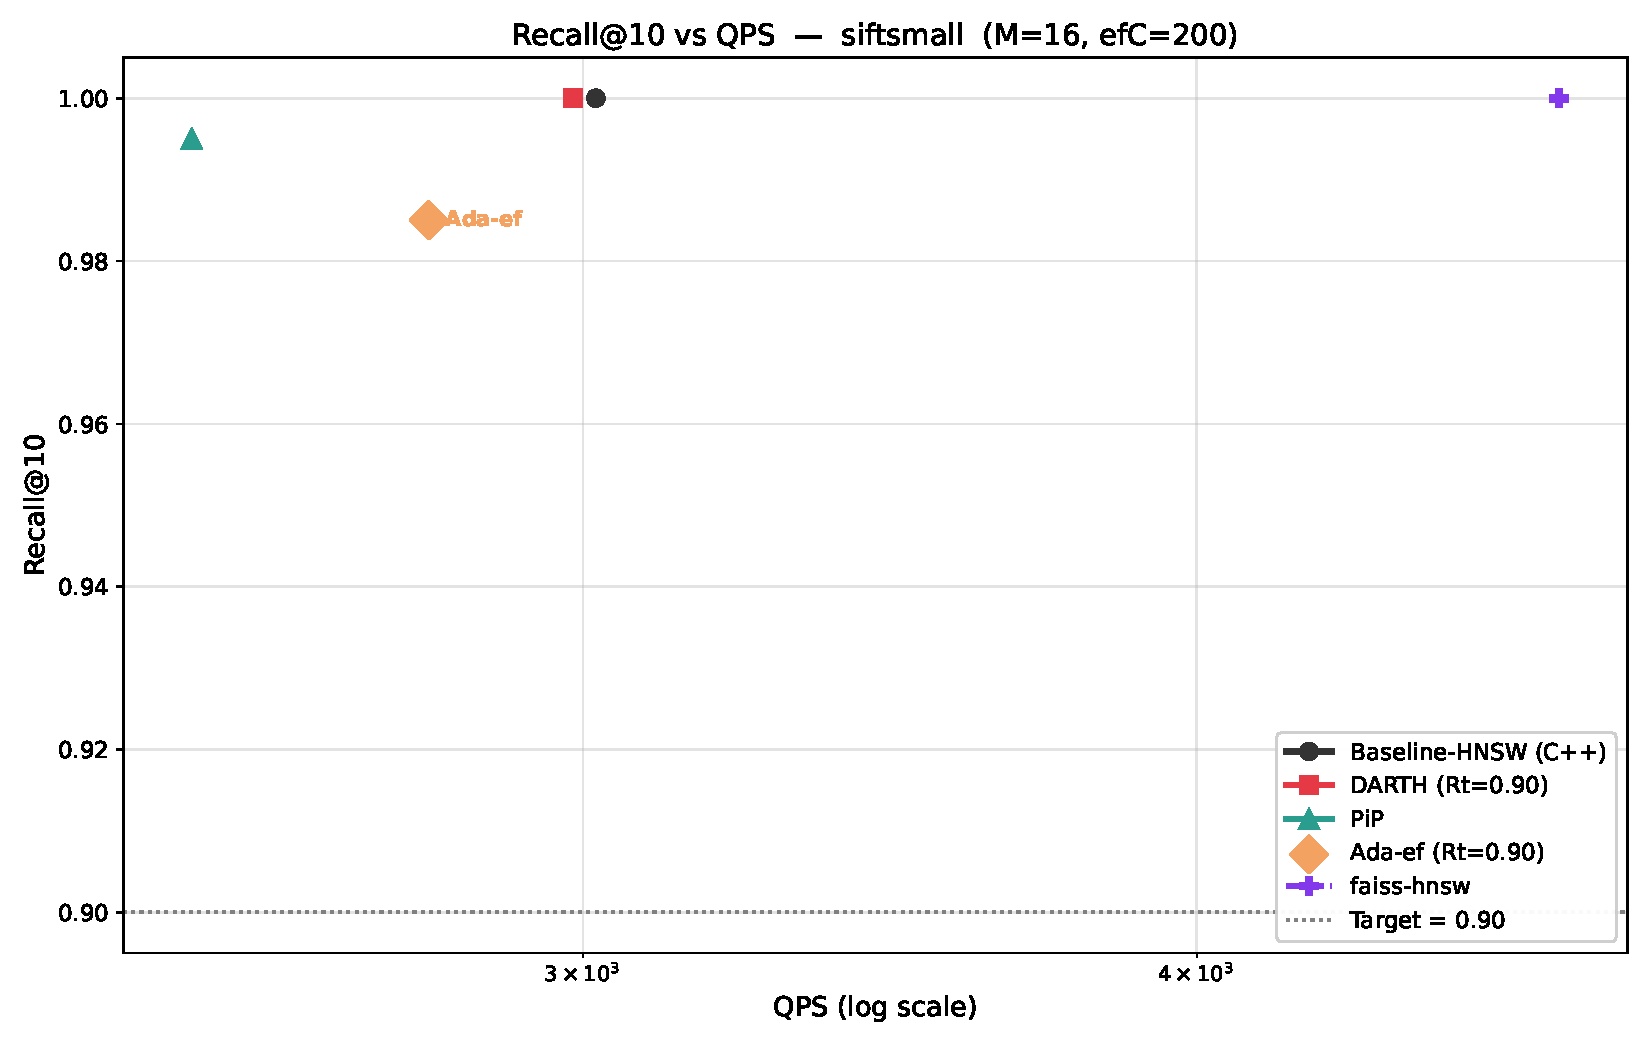
\includegraphics[width=\textwidth]{plots/recall_vs_qps_siftsmall.pdf}
        \caption{\selectlanguage{english}SIFT Small\selectlanguage{greek}}
    \end{subfigure}
    \hfill
    \begin{subfigure}[b]{0.48\textwidth}
        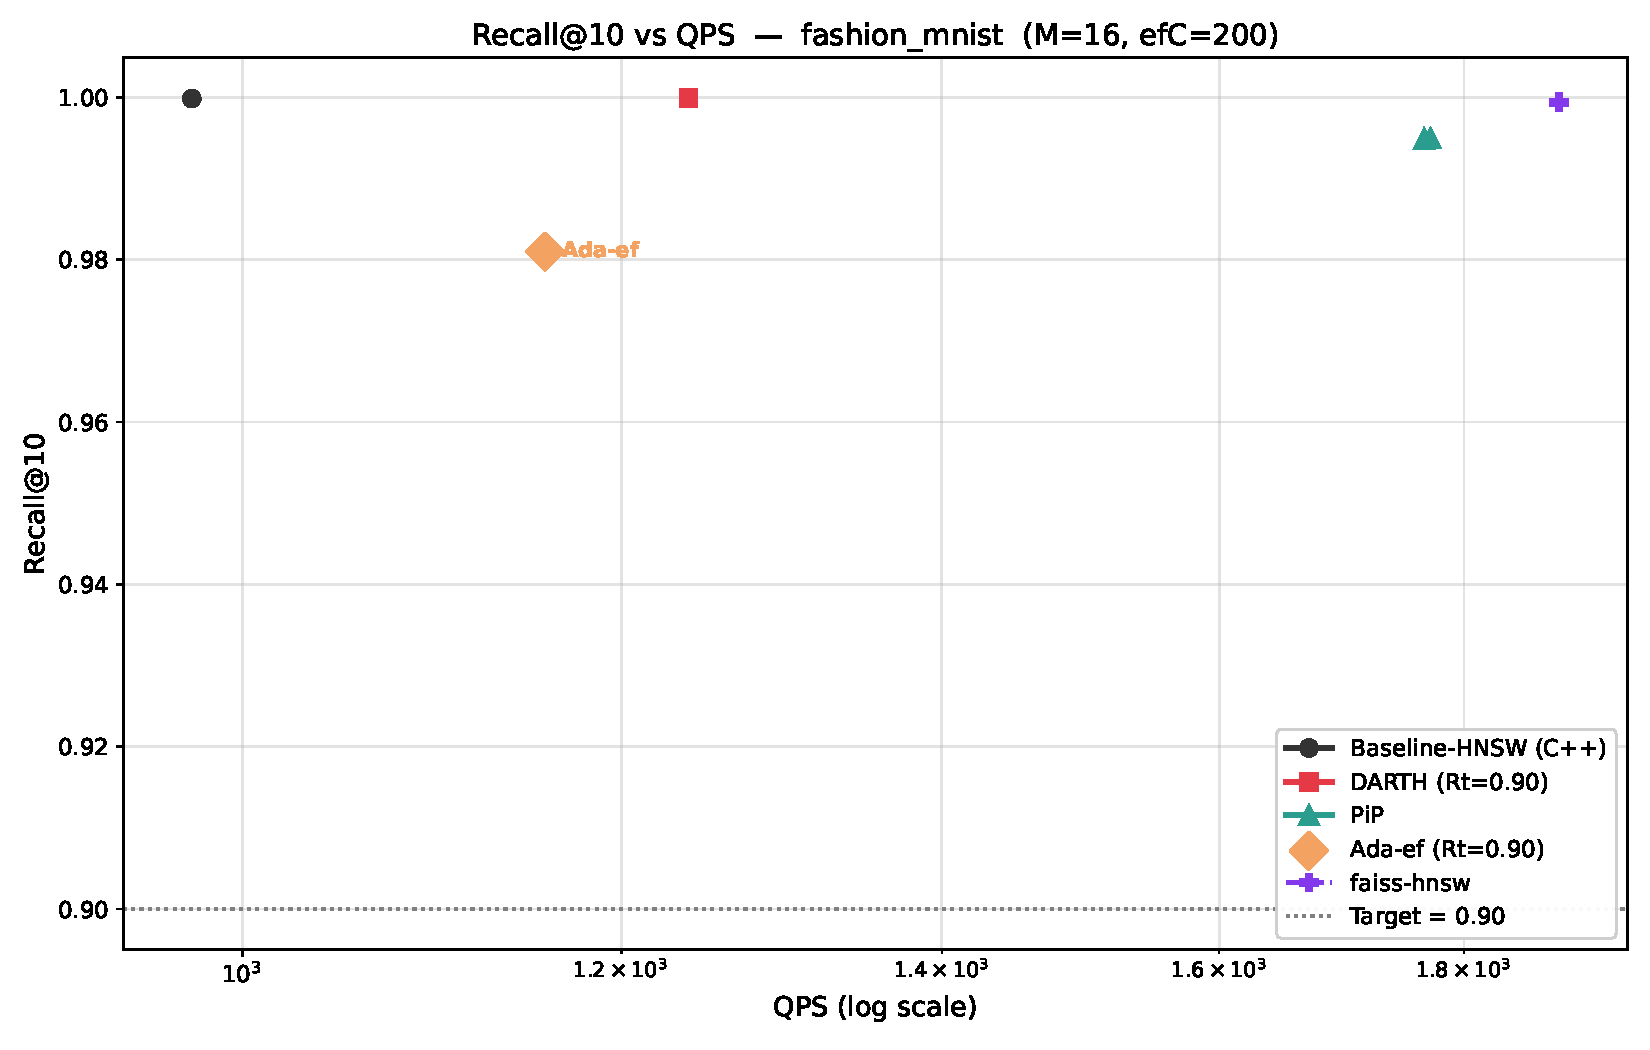
\includegraphics[width=\textwidth]{plots/recall_vs_qps_fashion_mnist.pdf}
        \caption{\selectlanguage{english}Fashion-MNIST\selectlanguage{greek}}
    \end{subfigure}
    \caption{\selectlanguage{english}Recall@10 vs QPS\selectlanguage{greek} για \selectlanguage{english}SIFT Small\selectlanguage{greek} και \selectlanguage{english}Fashion-MNIST\selectlanguage{greek} ($M=16$, $ef_C=200$, $k=10$)}
    \label{fig:qps_small}
\end{figure}

\begin{figure}[H]
    \centering
    \begin{subfigure}[b]{0.48\textwidth}
        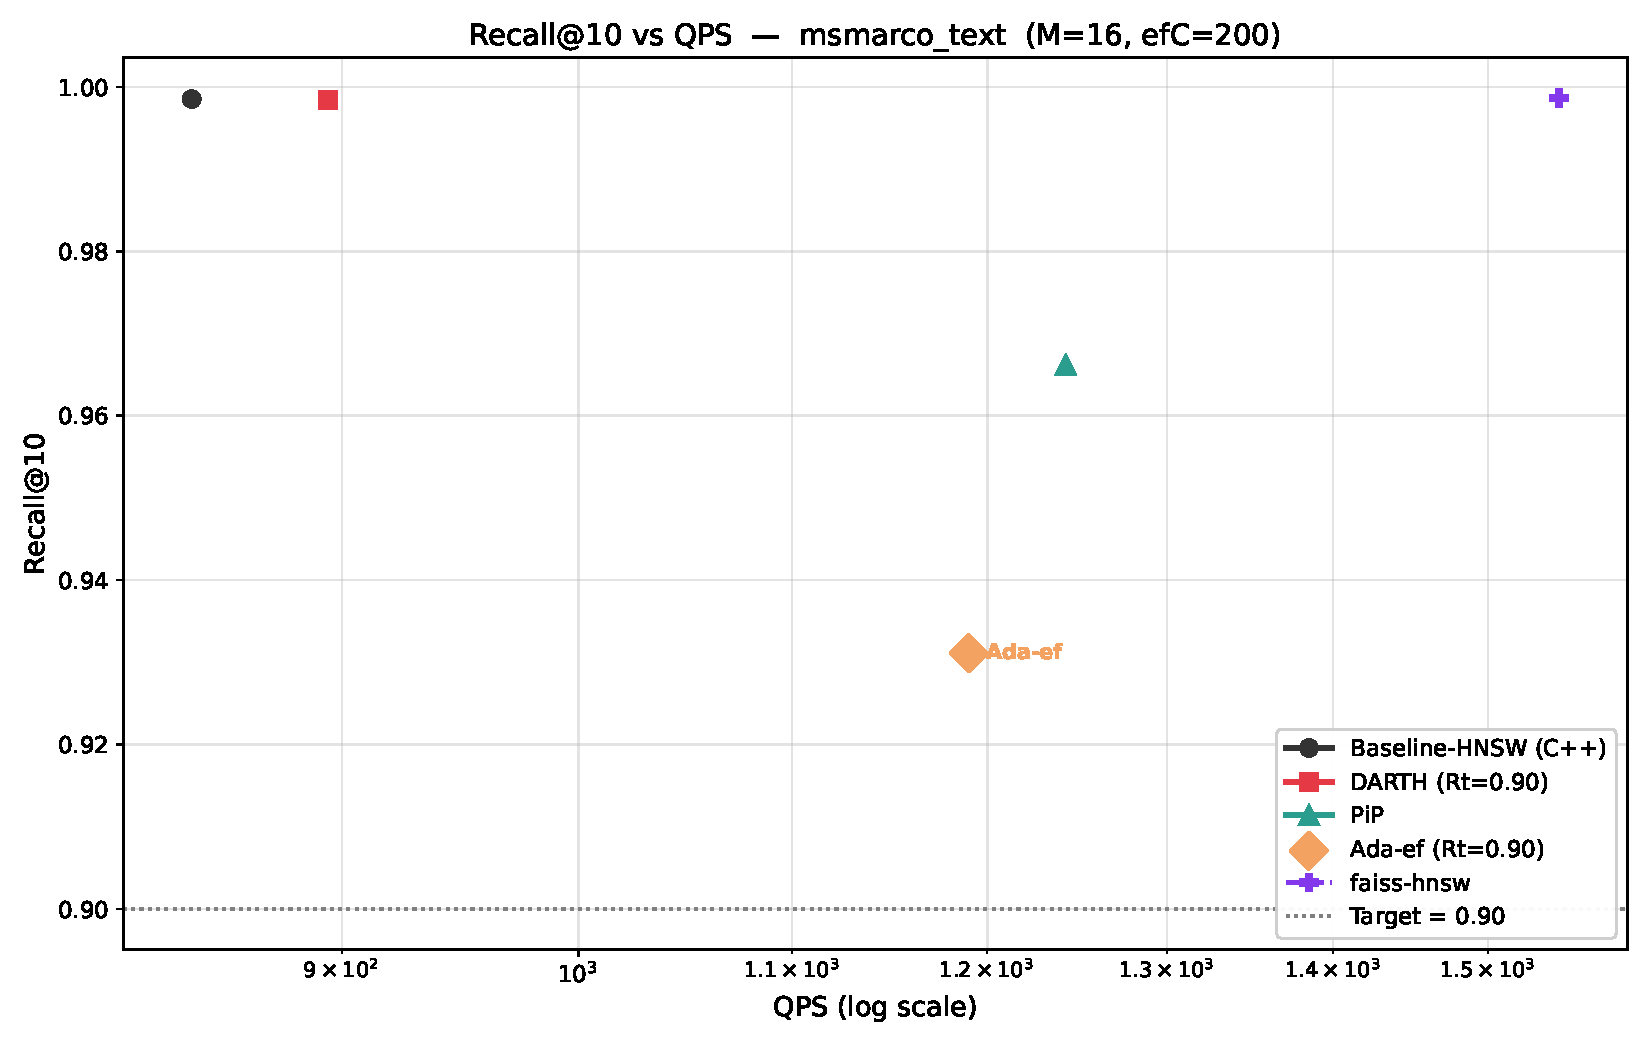
\includegraphics[width=\textwidth]{plots/recall_vs_qps_msmarco_text.pdf}
        \caption{\selectlanguage{english}MS MARCO Text\selectlanguage{greek}}
    \end{subfigure}
    \hfill
    \begin{subfigure}[b]{0.48\textwidth}
        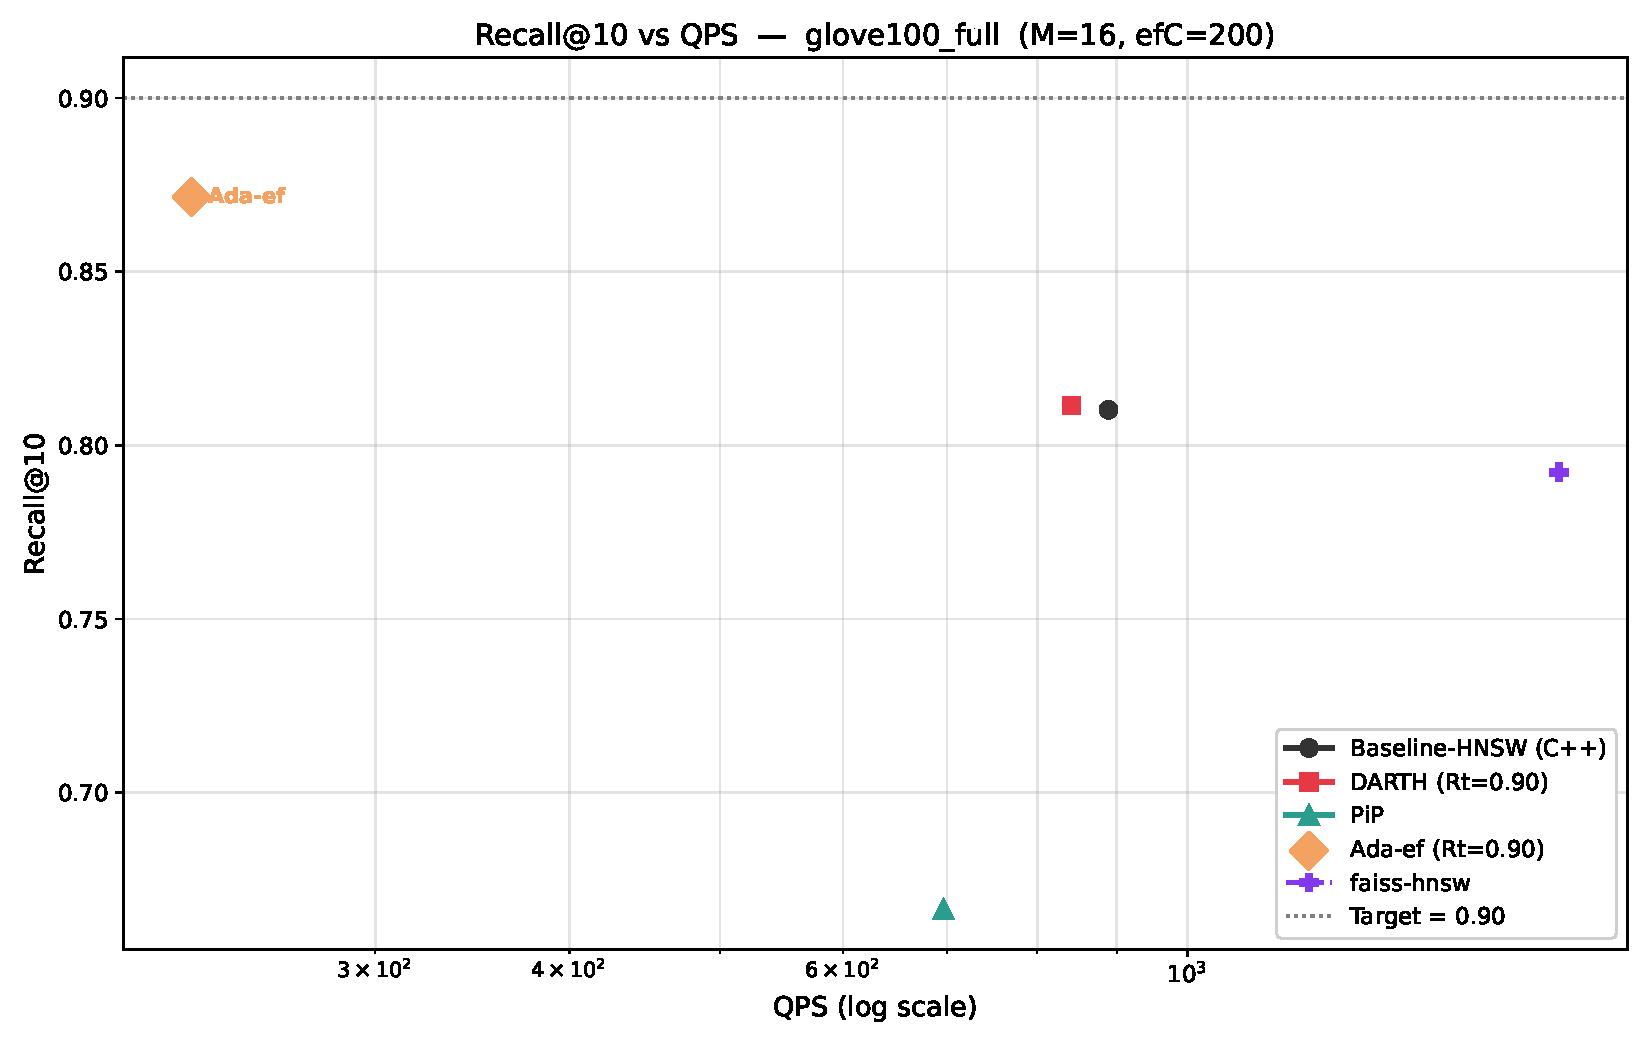
\includegraphics[width=\textwidth]{plots/recall_vs_qps_glove100_full.pdf}
        \caption{\selectlanguage{english}GloVe-100\selectlanguage{greek}}
    \end{subfigure}
    \caption{\selectlanguage{english}Recall@10 vs QPS\selectlanguage{greek} για \selectlanguage{english}MS MARCO Text\selectlanguage{greek} και \selectlanguage{english}GloVe-100\selectlanguage{greek} ($M=16$, $ef_C=200$, $k=10$)}
    \label{fig:qps_medium}
\end{figure}

\begin{figure}[H]
    \centering
    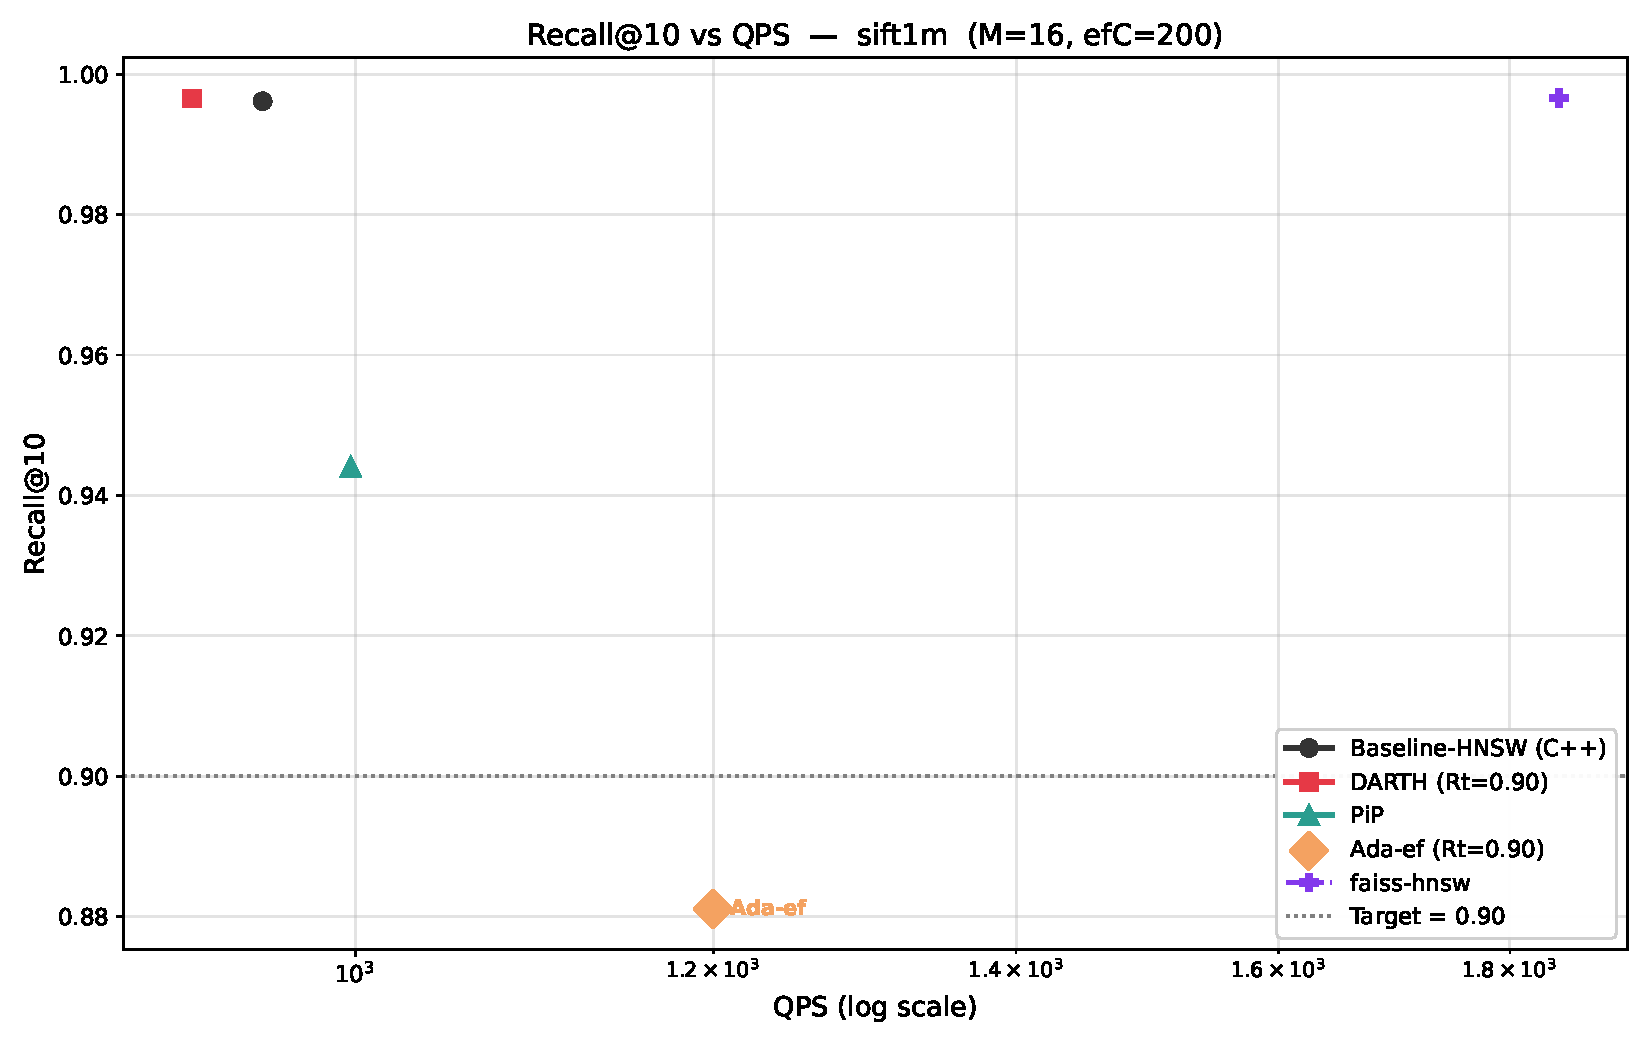
\includegraphics[width=0.55\textwidth]{plots/recall_vs_qps_sift1m.pdf}
    \caption{\selectlanguage{english}Recall@10 vs QPS\selectlanguage{greek} για \selectlanguage{english}SIFT-1M\selectlanguage{greek} ($M=16$, $ef_C=200$, $k=10$)}
    \label{fig:qps_sift1m}
\end{figure}

Ο Πίνακας~\ref{tab:results_main} συνοψίζει τα αποτελέσματα για αντιπροσωπευτικές τιμές $ef_{\text{search}} \in \{20, 100\}$, $M=16$, $ef_{\text{construction}}=200$, $k=10$.

\begin{table}[H]
\centering
\caption{Αποτελέσματα \selectlanguage{english}Recall@10 / QPS\selectlanguage{greek} για $M=16$, $ef_C=200$ ($ef_{\text{search}}=20$ και $ef_{\text{search}}=100$)}
\label{tab:results_main}
\resizebox{\textwidth}{!}{%
\begin{tabular}{llrrrr}
\toprule
\textbf{Dataset} & \textbf{Μέθοδος} & \multicolumn{2}{c}{$ef_{\text{search}}=20$} & \multicolumn{2}{c}{$ef_{\text{search}}=100$} \\
\cmidrule(lr){3-4} \cmidrule(lr){5-6}
 &  & Recall@10 & QPS & Recall@10 & QPS \\
\midrule
\multirow{4}{*}{SIFT Small}
  & Baseline-HNSW & 0.979 & 19.677 & 0.998 & 4.817 \\
  & DARTH         & 0.984 & 14.525 & 0.999 & 5.424 \\
  & PiP           & 0.982 & 4.143  & 0.995 & 2.621 \\
  & faiss-hnsw    & 0.980 & 35.745 & 1.000 & 9.677 \\
\midrule
\multirow{5}{*}{Fashion-MNIST}
  & Baseline-HNSW & 0.982 & 5.421  & 0.999 & 1.672 \\
  & DARTH         & 0.986 & 5.132  & 1.000 & 1.953 \\
  & PiP           & 0.982 & 2.594  & 0.995 & 1.808 \\
  & Ada-ef$^\dag$ & 0.981 & 1.157  & \multicolumn{2}{c}{---$^\dag$} \\
  & faiss-hnsw    & 0.981 & 9.003  & 0.999 & 3.105 \\
\midrule
\multirow{5}{*}{MS MARCO Text}
  & Baseline-HNSW & 0.900 & 6.727  & 0.993 & 1.400 \\
  & DARTH         & 0.905 & 5.457  & 0.994 & 1.409 \\
  & PiP           & 0.900 & 2.321  & 0.966 & 1.286 \\
  & Ada-ef$^\dag$ & 0.931 & 1.190  & \multicolumn{2}{c}{---$^\dag$} \\
  & faiss-hnsw    & 0.915 & 11.778 & 0.995 & 2.902 \\
\midrule
\multirow{5}{*}{GloVe-100}
  & Baseline-HNSW & 0.499 & 5.786  & 0.739 & 1.582 \\
  & DARTH         & 0.501 & 4.516  & 0.741 & 1.470 \\
  & PiP           & 0.493 & 1.751  & 0.665 & 0.761 \\
  & Ada-ef$^\dag$ & 0.871 & 0.229  & \multicolumn{2}{c}{---$^\dag$} \\
  & faiss-hnsw    & 0.485 & 10.988 & 0.722 & 2.989 \\
\midrule
\multirow{5}{*}{SIFT-1M}
  & Baseline-HNSW & 0.843 & 6.732  & 0.985 & 1.769 \\
  & DARTH         & 0.849 & 5.524  & 0.986 & 1.595 \\
  & PiP           & 0.841 & 2.037  & 0.944 & 1.043 \\
  & Ada-ef$^\dag$ & 0.881 & 1.200  & \multicolumn{2}{c}{---$^\dag$} \\
  & faiss-hnsw    & 0.853 & 12.200 & 0.987 & 3.401 \\
\bottomrule
\end{tabular}%
}
\smallskip

\noindent\footnotesize $^\dag$ Η \selectlanguage{english}Ada-ef\selectlanguage{greek} επιλέγει αυτόματα το \selectlanguage{english}efSearch\selectlanguage{greek} ανά ερώτημα μέσω \selectlanguage{english}offline\selectlanguage{greek} βαθμονόμησης· δεν εκτελείται για σταθερή τιμή $ef_{\text{search}}=100$ και επομένως δεν παράγει αποτελέσματα στη στήλη αυτή.
\end{table}

\subsection{Ανάλυση Αποτελεσμάτων}

\subsubsection{\selectlanguage{english}faiss-hnsw \selectlanguage{greek}ως Σημείο Αναφοράς}
Η \selectlanguage{english}faiss-hnsw\selectlanguage{greek} ήταν αναμενόμενα η πιο γρήγορη — 2 έως 5 φορές υψηλότερο \selectlanguage{english}QPS\selectlanguage{greek} σε σχέση με τη δική μας \selectlanguage{english}Baseline\selectlanguage{greek} σε όλα τα datasets. Αυτό δεν αποτελεί έκπληξη: το \selectlanguage{english}FAISS\selectlanguage{greek} είναι μια ώριμη βιβλιοθήκη με βαριές βελτιστοποιήσεις χαμηλού επιπέδου (\selectlanguage{english}SIMD\selectlanguage{greek}, \selectlanguage{english}cache-friendly memory layouts\selectlanguage{greek} κ.λπ.), ενώ η δική μας υλοποίηση στοχεύει στη σαφήνεια και την επεκτασιμότητα. Αξίζει να σημειωθεί ότι η \selectlanguage{english}faiss-hnsw\selectlanguage{greek} δεν έχει κανέναν προσαρμοστικό μηχανισμό — χρησιμοποιεί πάντα το ίδιο \selectlanguage{english}efSearch\selectlanguage{greek} για κάθε ερώτημα, οπότε η σύγκριση με τις προσαρμοστικές μεθόδους δεν είναι απόλυτα ισότιμη.

\subsubsection{\selectlanguage{english}DARTH\selectlanguage{greek}: Προσαρμοστική Πρόβλεψη Ανάκλησης}
Η \selectlanguage{english}DARTH\selectlanguage{greek} δεν είναι απλώς «καλύτερη ή χειρότερη» — εξαρτάται πολύ από τι ζητάς. Σε χαμηλά $ef_{\text{search}}$ (10--20) το \selectlanguage{english}QPS\selectlanguage{greek} της υποχωρεί κατά 20--30\% σε σχέση με τη \selectlanguage{english}Baseline\selectlanguage{greek}, επειδή το \selectlanguage{english}LightGBM\selectlanguage{greek} κοστίζει — και αν η αναζήτηση είναι ήδη σύντομη, αυτό το κόστος έχει βάρος. Αλλά στα υψηλά $ef_{\text{search}}$ (150--200) η εικόνα αλλάζει: η \selectlanguage{english}DARTH\selectlanguage{greek} σταματά νωρίτερα από τη \selectlanguage{english}Baseline\selectlanguage{greek} χωρίς να χάνει \selectlanguage{english}recall\selectlanguage{greek}, οπότε κερδίζει.

Το \selectlanguage{english}Fashion-MNIST\selectlanguage{greek} ήταν η καλύτερη περίπτωση. Πάνω από $ef_{\text{search}} = 50$, το \selectlanguage{english}Recall@10\selectlanguage{greek} σταθεροποιείται κοντά στο 0.999 — και η \selectlanguage{english}DARTH\selectlanguage{greek} το πετυχαίνει με λιγότερα βήματα. Προφανώς στο \selectlanguage{english}Fashion-MNIST\selectlanguage{greek} πολλά ερωτήματα «κλείνουν» γρήγορα, και το μοντέλο το πιάνει αυτό.

Στο \selectlanguage{english}GloVe-100\selectlanguage{greek} η \selectlanguage{english}DARTH\selectlanguage{greek} μένει οριακά μπροστά από τη \selectlanguage{english}Baseline\selectlanguage{greek} — 0.741 vs 0.739 για $ef_{\text{search}}=100$ — αλλά με χαμηλότερο \selectlanguage{english}QPS\selectlanguage{greek}. Το dataset αυτό είναι δύσκολο για όλες τις μεθόδους: τα διανύσματα λέξεων είναι ομοιόμορφα κατανεμημένα στον χώρο, οπότε ο πρόωρος τερματισμός σπάνια ενεργοποιείται — κάθε ερώτημα απαιτεί εξερεύνηση.

Στο \selectlanguage{english}SIFT-1M\selectlanguage{greek} — 1 εκατομμύριο διανύσματα — η \selectlanguage{english}DARTH\selectlanguage{greek} κρατάει τη θέση της: 0.986 \selectlanguage{english}Recall@10\selectlanguage{greek} έναντι 0.985 της \selectlanguage{english}Baseline\selectlanguage{greek} για $ef_{\text{search}}=100$, με \selectlanguage{english}QPS\selectlanguage{greek} 1.595 έναντι 1.769. Δεν είναι δραματική διαφορά, αλλά το σημαντικό είναι ότι ο \selectlanguage{english}predictor\selectlanguage{greek} εξακολουθεί να λειτουργεί σωστά σε αυτή την κλίμακα.

\subsubsection{\selectlanguage{english}PiP\selectlanguage{greek}: Κλάδεμα Υποψηφίων}
Η \selectlanguage{english}PiP\selectlanguage{greek} ήταν η πιο απογοητευτική μέθοδος. Σε κανένα dataset δεν ξεπέρασε τη \selectlanguage{english}Baseline-HNSW\selectlanguage{greek} σε \selectlanguage{english}QPS\selectlanguage{greek} — και αυτό συνοδεύεται από ένα ακόμα βαθύτερο πρόβλημα. Πάνω από $ef_{\text{search}} \approx 50$, το \selectlanguage{english}recall\selectlanguage{greek} απλώς σταματά να βελτιώνεται. Αυξάνεις το \selectlanguage{english}budget\selectlanguage{greek} αναζήτησης, πληρώνεις περισσότερο — και δεν παίρνεις τίποτα πίσω.

Στο \selectlanguage{english}SIFT-1M\selectlanguage{greek} αυτό φαίνεται καθαρά: το \selectlanguage{english}Recall@10\selectlanguage{greek} κολλάει στο 0.944 για $ef_{\text{search}} \geq 100$, ενώ η \selectlanguage{english}Baseline\selectlanguage{greek} φτάνει 0.985. Στο \selectlanguage{english}GloVe-100\selectlanguage{greek} το ίδιο πρόβλημα — κορεσμός στο 0.665 για $ef_{\text{search}}=100$, όταν η \selectlanguage{english}Baseline\selectlanguage{greek} φτάνει 0.739. Μάλλον το κλάδεμα υποψηφίων αποκλείει διαδρομές που σε μεγάλες βάσεις είναι απαραίτητες για να βρεθούν οι σωστοί γείτονες.

\subsubsection{\selectlanguage{english}Ada-ef\selectlanguage{greek}: Προσαρμοστικό \selectlanguage{english}efSearch\selectlanguage{greek}}
Η \selectlanguage{english}Ada-ef\selectlanguage{greek} έχει μια ιδιαιτερότητα που αξίζει να αναφερθεί: τρέχει με \selectlanguage{english}cosine similarity\selectlanguage{greek} — μετά από \selectlanguage{english}L2\selectlanguage{greek} κανονικοποίηση — ενώ όλες οι άλλες μέθοδοι χρησιμοποιούν ευκλείδεια απόσταση. Δεν είναι ακριβώς ισότιμη σύγκριση, και το λέμε ξεκάθαρα.

Στο \selectlanguage{english}SIFT-1M\selectlanguage{greek} έδωσε \selectlanguage{english}Recall@10\selectlanguage{greek} = 0.881 με \selectlanguage{english}QPS\selectlanguage{greek} = 1.200 — αξιοπρεπές \selectlanguage{english}recall\selectlanguage{greek}, αλλά αισθητά χαμηλότερο \selectlanguage{english}QPS\selectlanguage{greek} από τη \selectlanguage{english}Baseline\selectlanguage{greek} στο ίδιο επίπεδο ανάκλησης. Η \selectlanguage{english}offline\selectlanguage{greek} βαθμονόμηση είναι ακριβή — και σε 1 εκατομμύριο διανύσματα αυτό φαίνεται.

\subsubsection{Επίδραση Παραμέτρων $M$ και $ef_{\text{construction}}$}
Αυξάνοντας το $M$ από 8 σε 16, παρατηρήσαμε βελτίωση 2--5\% στο \selectlanguage{english}Recall@10\selectlanguage{greek} για τα μεγαλύτερα datasets (\selectlanguage{english}GloVe-100, SIFT-1M\selectlanguage{greek}), με το αντίτιμο αύξησης του χρόνου κατασκευής — που στο \selectlanguage{english}SIFT-1M\selectlanguage{greek} φτάνει τις 4.400 δευτερόλεπτα και στο \selectlanguage{english}GloVe-100\selectlanguage{greek} τις 5.000. Για το $ef_{\text{construction}}$, η μετακίνηση από 128 σε 200 είχε μικρότερη επίδραση στην ανάκληση από ό,τι αρχικά περιμέναμε, αλλά αύξησε σαφώς τον χρόνο κατασκευής — έως $\times 1.5$ σε μερικές περιπτώσεις. Στο \selectlanguage{english}SIFT Small\selectlanguage{greek} οι δύο ρυθμίσεις έδωσαν σχεδόν πανομοιότυπα αποτελέσματα, κάτι που έχει νόημα δεδομένου του πολύ μικρού μεγέθους του dataset.

% =======================================
% Συμπεράσματα και Μελλοντική Εργασία: ΚΕΦΑΛΑΙΟ 6
% =======================================
\newpage
\section{Συμπεράσματα και Μελλοντική Εργασία}

\subsection{Συμπεράσματα}

Η εργασία αυτή ξεκίνησε από ένα απλό ερώτημα: αξίζει να προσθέσουμε πολυπλοκότητα στον \selectlanguage{english}HNSW\selectlanguage{greek} — είτε υπό μορφή προσαρμοστικής αναζήτησης, είτε κλαδέματος — και αν ναι, πού;

Η σύντομη απάντηση είναι ότι εξαρτάται. Η \selectlanguage{english}DARTH\selectlanguage{greek} λειτούργησε καλά σε datasets με ετερογενή δυσκολία ερωτημάτων — χαρακτηριστικά το \selectlanguage{english}Fashion-MNIST\selectlanguage{greek} — όπου η πρόβλεψη του \selectlanguage{english}LightGBM\selectlanguage{greek} επιτρέπει πρόωρο τερματισμό και διατηρεί υψηλό \selectlanguage{english}recall\selectlanguage{greek}. Στο \selectlanguage{english}GloVe-100\selectlanguage{greek} όμως — 1,18 εκατομμύρια διανύσματα λέξεων με ομοιόμορφη κατανομή — το πλεονέκτημα σχεδόν εξαφανίζεται. Αυτό που ίσως εκπλήσσει είναι ότι στο \selectlanguage{english}SIFT-1M\selectlanguage{greek} ο \selectlanguage{english}predictor\selectlanguage{greek} κλιμακώνεται κανονικά.

Η \selectlanguage{english}PiP\selectlanguage{greek} δεν ανταποκρίθηκε στις προσδοκίες. Σε καμία περίπτωση δεν ξεπέρασε τη \selectlanguage{english}Baseline\selectlanguage{greek}, και στο \selectlanguage{english}SIFT-1M\selectlanguage{greek} ο κορεσμός ανάκλησης είναι ακόμα πιο έντονος: το \selectlanguage{english}Recall@10\selectlanguage{greek} αρνείται να ανέβει πάνω από 0.944, ενώ η \selectlanguage{english}Baseline\selectlanguage{greek} φτάνει 0.985. Αυτό δείχνει δομικό πρόβλημα, όχι απλώς κακή ρύθμιση παραμέτρων.

Για τη \selectlanguage{english}Ada-ef\selectlanguage{greek}, τα πράγματα είναι πιο σύνθετα επειδή λειτουργεί με \selectlanguage{english}cosine similarity\selectlanguage{greek} αντί \selectlanguage{english}L2\selectlanguage{greek} — δεν είναι ισότιμη σύγκριση. Στο \selectlanguage{english}GloVe-100\selectlanguage{greek} πετυχαίνει \selectlanguage{english}Recall@10\selectlanguage{greek} = 0.871 — αισθητά υψηλότερο από τη \selectlanguage{english}Baseline\selectlanguage{greek} (0.739) στο ίδιο \selectlanguage{english}budget\selectlanguage{greek}. Αυτό έχει νόημα: το \selectlanguage{english}GloVe-100\selectlanguage{greek} χρησιμοποιείται κανονικά με \selectlanguage{english}cosine similarity\selectlanguage{greek}, οπότε η \selectlanguage{english}Ada-ef\selectlanguage{greek} παίζει στο δυνατό της. Το τίμημα είναι \selectlanguage{english}QPS\selectlanguage{greek} = 229 — πολύ αργή για παραγωγικό σύστημα. Στο \selectlanguage{english}SIFT-1M\selectlanguage{greek} επιτυγχάνει \selectlanguage{english}Recall@10\selectlanguage{greek} = 0.881 με \selectlanguage{english}QPS\selectlanguage{greek} = 1.200, αλλά πάλι χαμηλότερη ταχύτητα από τη \selectlanguage{english}Baseline\selectlanguage{greek} για παρόμοιο \selectlanguage{english}recall\selectlanguage{greek}.

Τέλος, η \selectlanguage{english}faiss-hnsw\selectlanguage{greek} επιβεβαίωσε ότι οι χαμηλού επιπέδου βελτιστοποιήσεις — \selectlanguage{english}SIMD\selectlanguage{greek}, \selectlanguage{english}cache-friendly layouts\selectlanguage{greek} — κάνουν μεγάλη διαφορά σε πρακτικά σενάρια. Το χάσμα 2--5$\times$ σε \selectlanguage{english}QPS\selectlanguage{greek} έναντι της δικής μας \selectlanguage{english}Baseline\selectlanguage{greek} δεν οφείλεται σε αλγοριθμικές διαφορές αλλά σε υλοποιητικές. Αυτό δείχνει ότι για παραγωγικά συστήματα, το «πού τρέχεις» έχει εξίσου σημασία με το «πώς αναζητάς».

\subsection{Μελλοντική Εργασία}

Κάποια ερωτήματα που προέκυψαν κατά τη διεξαγωγή της εργασίας και παραμένουν ανοιχτά:

\begin{itemize}
    \item Το μοντέλο \selectlanguage{english}DARTH\selectlanguage{greek} εκπαιδεύτηκε \selectlanguage{english}offline\selectlanguage{greek} με σταθερό σύνολο χαρακτηριστικών. Θα ήταν ενδιαφέρον να δοκιμαστεί μια \selectlanguage{english}online\selectlanguage{greek} παραλλαγή που προσαρμόζεται δυναμικά στη στατιστική των ερωτημάτων, ή να αντικατασταθεί το \selectlanguage{english}LightGBM\selectlanguage{greek} με ένα ελαφρύτερο νευρωνικό δίκτυο.

    \item Όλες οι μέθοδοι αξιολογήθηκαν σε στατικά datasets. Σε πραγματικές βάσεις δεδομένων διανυσμάτων οι εισαγωγές και διαγραφές είναι συνεχείς — αξίζει να εξεταστεί πώς συμπεριφέρονται οι προσαρμοστικές στρατηγικές υπό δυναμικές συνθήκες.

    \item Η αξιολόγηση επεκτάθηκε μέχρι 1.000.000 διανύσματα (\selectlanguage{english}SIFT-1M\selectlanguage{greek}), όπου η \selectlanguage{english}DARTH\selectlanguage{greek} αποδείχθηκε αποτελεσματική. Η επόμενη φυσική κλιμάκωση — δισεκατομμύρια διανύσματα (\selectlanguage{english}SIFT-1B\selectlanguage{greek}) — παραμένει ανοιχτό ερώτημα, ιδιαίτερα για το κόστος κατασκευής του \selectlanguage{english}index\selectlanguage{greek} και εκπαίδευσης του \selectlanguage{english}predictor\selectlanguage{greek}.

    \item Η \selectlanguage{english}PiP\selectlanguage{greek} έδειξε κορεσμό ανάκλησης που δεν αναλύσαμε σε βάθος. Μια πιο λεπτομερής ανάλυση της δομής του γράφου που κατασκευάζει — σε σχέση με τον \selectlanguage{english}Baseline\selectlanguage{greek} — θα μπορούσε να φωτίσει γιατί το επιπλέον \selectlanguage{english}budget\selectlanguage{greek} αναζήτησης δεν μεταφράζεται σε βελτίωση.
\end{itemize}

% =======================================
% ΠΑΡΑΡΤΗΜΑΤΑ
% =======================================
\clearpage
\appendix

% Αν θες να εμφανίζονται στα Περιεχόμενα (ToC)
\section*{Παράρτημα Ι: Μεγάλοι Πίνακες Δεδομένων}
\addcontentsline{toc}{section}{Παράρτημα Ι: Μεγάλοι Πίνακες Δεδομένων}

Στο παράρτημα αυτό παρατίθενται αναλυτικά οι μεγάλοι πίνακες δεδομένων
που χρησιμοποιήθηκαν στα πειράματα.

\begin{table}[h!]
    \centering
    \caption{Ενδεικτικός μεγάλος πίνακας αποτελεσμάτων}
    \begin{tabular}{lccc}
        \toprule
        Μέθοδος & Recall@10 & Χρόνος Αναζήτησης (ms) & Μνήμη (MB) \\
        \midrule
        Δική μας HNSW υλοποίηση & 0.93 & 1.25 & 512 \\
        HNSWlib & 0.95 & 0.98 & 540 \\
        FAISS HNSW & 0.94 & 1.05 & 500 \\
        \bottomrule
    \end{tabular}
\end{table}


\clearpage
\section*{Παράρτημα ΙΙ: Κώδικας}
\addcontentsline{toc}{section}{Παράρτημα ΙΙ: Κώδικας}

Εδώ παρατίθενται μεγάλα αποσπάσματα κώδικα τα οποία δεν χωρούσαν
στο κύριο σώμα της εργασίας.

\begin{lstlisting}[language=Python, caption={Ενδεικτικό απόσπασμα κώδικα HNSW}]
class HNSWIndex:
    def __init__(self, m=16, ef_construction=200):
        self.m = m
        self.ef_construction = ef_construction
        self.layers = []
        # ...

    def add_point(self, vector, label):
        # υλοποίηση εισαγωγής κόμβου στο γράφο HNSW
        pass
\end{lstlisting}


\clearpage
\section*{Παράρτημα ΙΙΙ: Πρόσθετα Διαγράμματα}
\addcontentsline{toc}{section}{Παράρτημα ΙΙΙ: Πρόσθετα Διαγράμματα}

Στο παράρτημα αυτό δίνονται επιπλέον διαγράμματα από τα πειράματα.

\begin{figure}[h!]
    \centering
    % Αντικατέστησε το example-image με το δικό σου αρχείο
    
    \caption{Ενδεικτικό επιπλέον διάγραμμα αποτελεσμάτων.}
\end{figure}


% =======================================
% ΒΙΒΛΙΟΓΡΑΦΙΑ (IEEE style)
% =======================================
\clearpage


\renewcommand{\refname}{Βιβλιογραφικές Αναφορές}


\bibliographystyle{IEEEtran}
\bibliography{references/bibliography}
  



\end{document}
